Top-quark pair production events in which at least one \tauhadvis candidate
originates from a misidentified quark- or gluon-initiated jet are the
second-largest background in the \hadhad channel. A fraction of
\SI{85}{\percent} of events from this background stem from semi-leptonic decay
modes of \ttbar. In these events, the selected \tauhadvis candidates consist of
one true- and one \faketauhadvis. The remaining \SI{15}{\percent} are
\ttbarFakes events with two \faketauhadvis.
% The fraction of \ttbarFakes events with both candidates being \faketauhadvis
% is about \SI{15}{\percent} and thus comparatively small.
The \ttbarFakes background is estimated using simulation after applying
data-driven corrections in the form of \faketauhadvis scale factors (SFs)
measured in a CR enriched in \ttbar events. The SFs correct the \jettotauhadvis
misidentification efficiencies predicted by simulation, which are not centrally
calibrated by the ATLAS collaboration due to their process dependency.

Before proceeding with the description of the method, differences between
\faketauhadvis backgrounds from \ttbar and multi-jet are highlighted that
motivate the use of different background estimation techniques:
\begin{itemize}

\item The majority of \ttbarFakes background events consist of only one
  \faketauhadvis, while in multi-jet events both candidates are \faketauhadvis.

\item The probability that a quark- or gluon-initiated jet reconstructed as a
  \tauhadvis passes \tauid, also called the \emph{fake rate}, depends on the
  type of parton that initiated the jet. In \ttbar events, \faketauhadvis
  predominately originate from quarks produced in decays of $W$~bosons, which
  have larger fake rates than gluon-initiated jets. As a result, \faketauhadvis
  background estimation is inherently process dependent.

\item In the \hadhad channel, no suitable \ttbarFakes CR can be defined that
  separates \faketauhadvis backgrounds from \ttbar and multi-jet while
  maintaining sufficient statistical precision for background estimation. This
  necessitates defining a CR in $\ell + \tauhadvis$ ($\ell = e, \mu$) final
  states in which the multi-jet contribution can be neglected.

\end{itemize}
The main disadvantage of separately estimating the \faketauhadvis background
from \ttbar and multi-jet is the inflation of systematic uncertainties on the
estimate of the total \faketauhadvis background compared to a combined
approach.\footnote{An example of a combined approach is the combined fake factor
  method employed in the \lephad channel. This method is summarised
  in~\Cref{sec:bkg_lephad_combined_ff}.}  However, these inflated uncertainties
have little effect on the signal sensitivity for two reasons: First, the
targeted signal processes have distinct kinematic properties that differentiate
them from \faketauhadvis backgrounds. Second, the search is limited by
statistical uncertainties as opposed to systematic ones.


\subsubsection{Control Region Definition}

The CR for the SF measurement (SF-CR) targets final states with an electron or
muon and a \tauhadvis candidate. The region definition is based on the
selections applied in the \lephad channels, where a similar CR is used for
\faketauhadvis background estimation. Minor changes are applied to its
definition to ensure consistency with the SR selection of the \hadhad
channel. The most important selection criteria and differences are briefly
summarised:
\begin{itemize}

\item The \tauhadvis selection is adapted to follow the selection of the \hadhad
  channel more closely by selecting candidates with $\pT > \SI{25}{\GeV}$ and
  $|\eta| < \num{2.5}$ (instead of $\pT > \SI{20}{\GeV}$ and
  $|\eta| < \num{2.3}$ in the \lephad channels).

\item All events are required to have exactly one \tauhadvis candidate passing
  \tauid, exactly one electron or muon passing their respective isolation and
  identification criteria, and exactly two \btagged jets. In addition, only
  events passing the SLT selection are considered.

\item The electron/muon and the \tauhadvis candidate are required to be
  reconstructed with electric charges of opposite sign.
  % This requirement ensures that the charge correlations between light lepton
  % and \faketauhadvis from semi-leptonic decays of \ttbar are similar to the
  % correlation between \tauhadvis candidates from \ttbarFakes in the \hadhad SR
  % for cases where only one candidate is a \faketauhadvis. The effect of charge
  % correlation on \ttbarFakes estimation was previously studied in
  % Ref.~\cite{bokan}.

\item Orthogonality between the SF-CR and the SR of the \lephad SLT channel is
  ensured by requiring $\mBB > \SI{150}{\GeV}$.

\end{itemize}

% \footnote{Leptons $\ell$ and true \tauhadvis are have high
% probability to be reconstructed with the correct electric charge in
% the SF-CR. In \ttbar the \faketauhadvis candidate is more likely to
% have opposite-sign electric charge . As a result, in the same-sign
% region the quark/gluon composition of jets is likely different which
% also affects the fake rates.}.

The dominant process populating the SF-CR is \ttbar production, which is
selected with a purity of \SI{94}{\percent}. About \SI{66}{\percent} of SF-CR
events are from di-leptonic decay modes of \ttbar that yield an electron/muon
and a \tauhadvis in the final state. The production of \ttbar events with
\tauhadvis candidates originating from quark- or gluon-initiated jets, which is
the process of interest for this measurement, constitutes \SI{28}{\percent} of
selected events. Minor backgrounds in this region are single-top-quark
(\SI{4}{\percent}) and $\Vjets$ (\SI{2}{\percent}) production. The \multijet
background is assumed to be negligible. The distribution of transverse momenta
and pseudorapidity of \tauhadvis candidates in the SF-CR prior to the fit is
shown in~\Cref{fig:ttbarSF_prefit_pt}.

\begin{figure}[htbp]
  \centering

  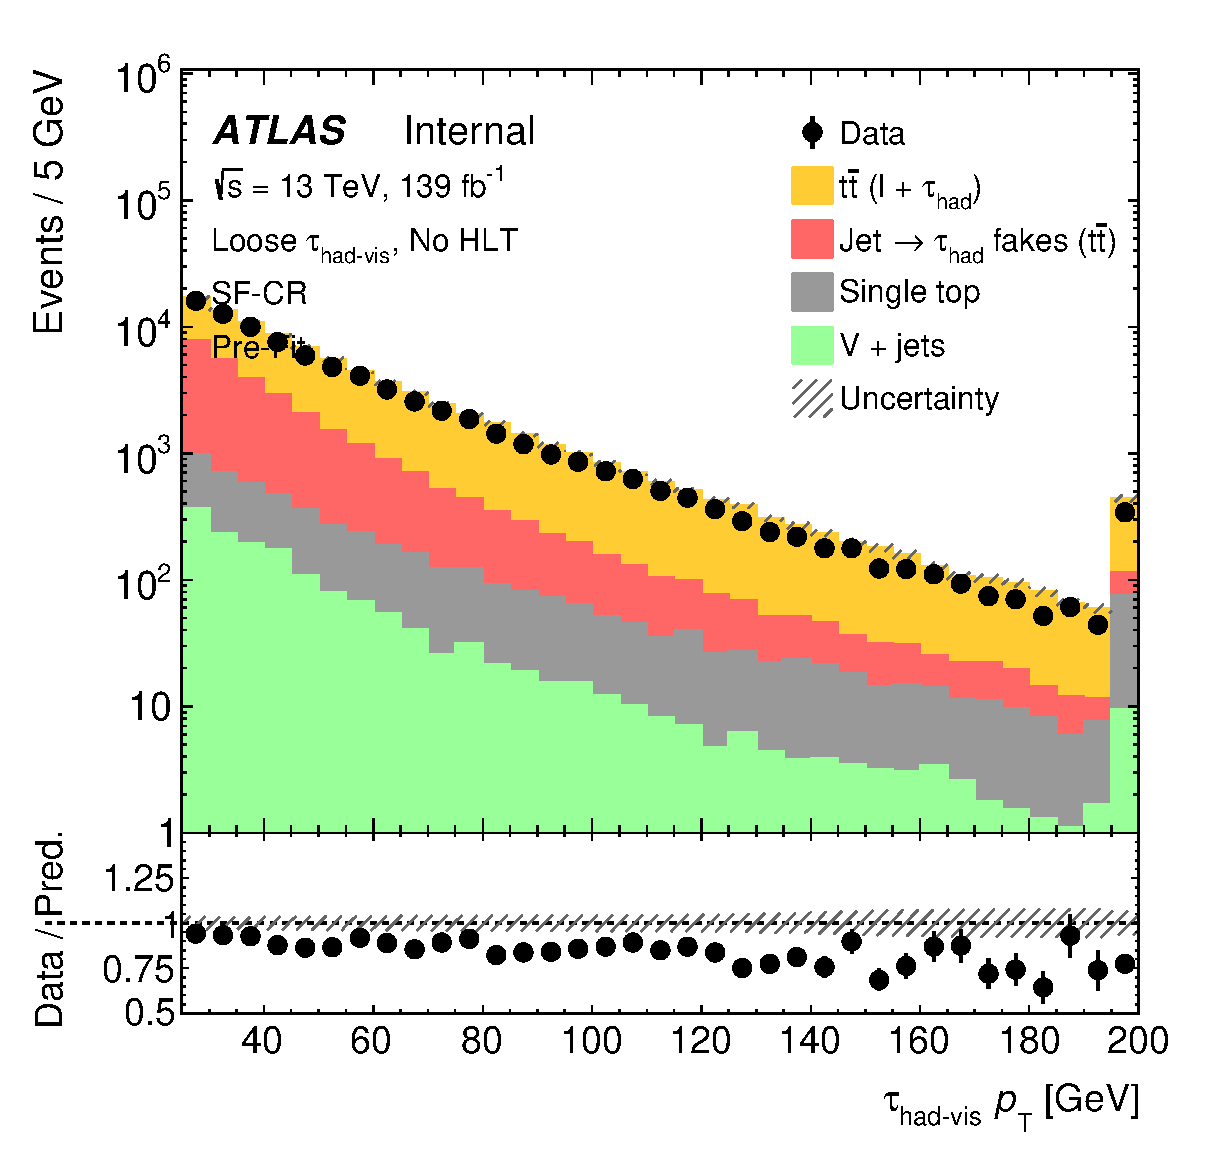
\includegraphics[width=0.49\textwidth]{ttbarSF/prefit_sfcr/PTVR}%
  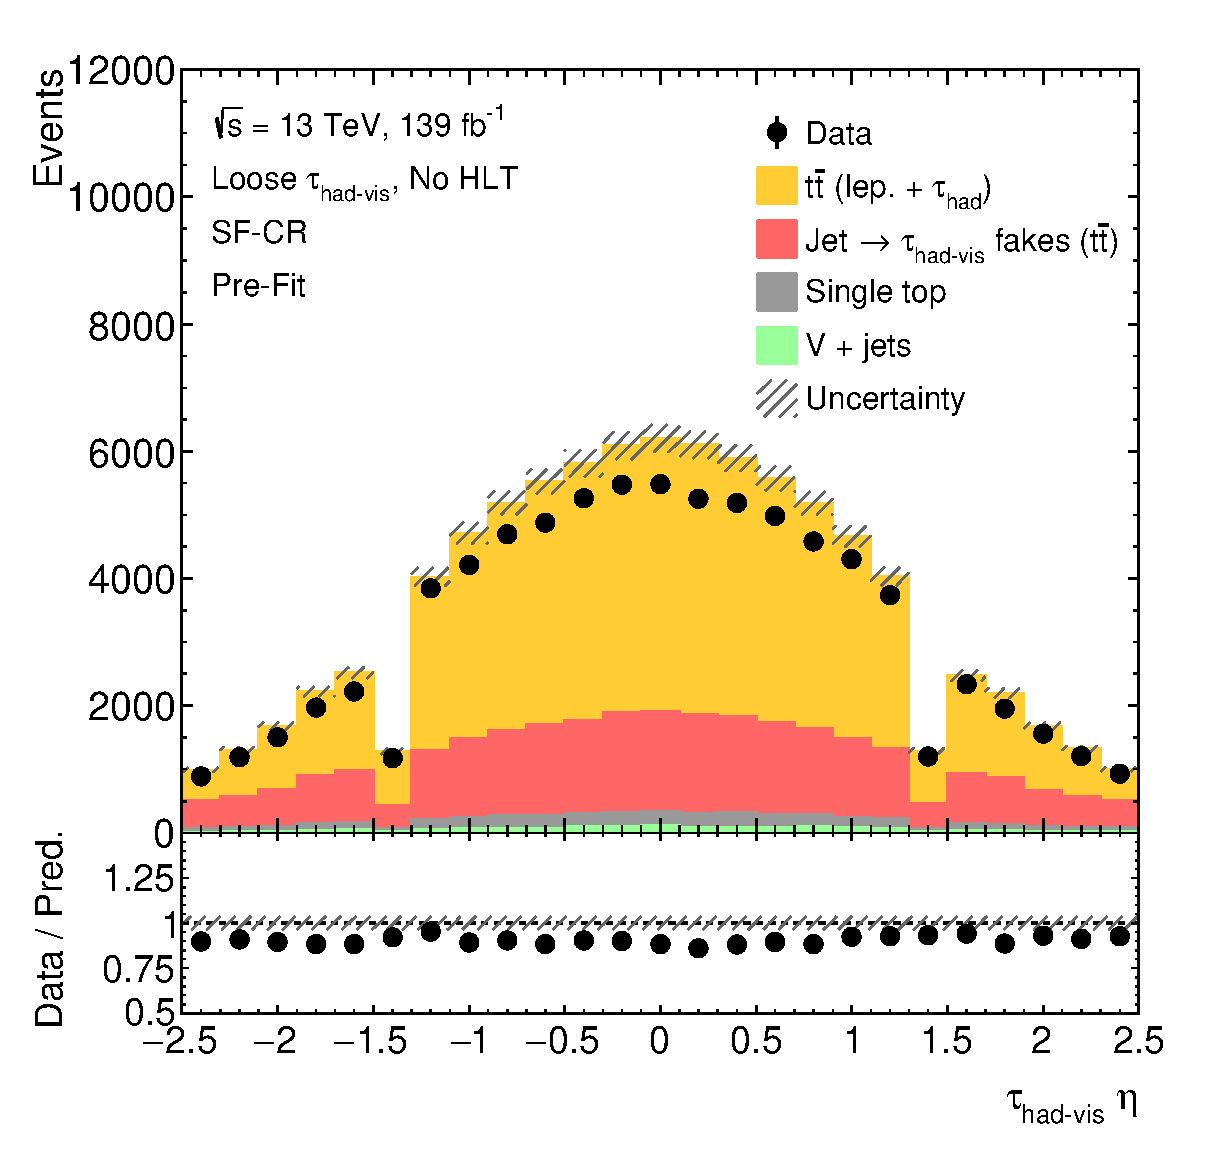
\includegraphics[width=0.49\textwidth]{ttbarSF/prefit_sfcr/ETAVR}

  \caption[Distribution of \tauhadvis \pT and $\eta$ in the SF-CR.]{Distribution
    of \tauhadvis \pT and $\eta$ in the SF-CR prior to the fit. Events with
    \tauhadvis candidate \pT larger than \SI{200}{\GeV} are included in the last
    bin. All statistical and systematic uncertainties are included.}%
  \label{fig:ttbarSF_prefit_pt}
\end{figure}

\Jettotauhadvis misidentification efficiencies depend on the identification
requirements applied to \tauhadvis candidates. In this search, such requirements
are imposed on \tauhadvis candidates at trigger-level and during offline event
reconstruction. This two-stage selection of \tauhadvis candidates is taken into
account by measuring separate sets of SFs for every relevant combination of
\tauid requirements. One set of SFs is measured for \faketauhadvis after offline
\tauid but without requirements at trigger-level.
% These SFs are required for STT events in the \hadhad channel in cases where
% the \faketauhadvis was not the candidate causing the trigger to select the
% event.
Three sets of SFs are measured to account for identification requirements
applied at trigger-level and during offline event reconstruction.
% chains used in the \hadhad channel (cf.~\Cref{sec:hadhad_trigger_selection})
% which are applied in addition to offline \tauid.

The measurement of SFs without requirements at trigger-level can proceed using
events in the SF-CR without additional selections. For measurements of SFs that
include trigger-level identification requirements, the selections applied by
\tauhadvis-triggers need to be emulated. This is achieved by requiring that
events in the SF-CR are also selected by appropriately chosen single-\tauhadvis
triggers. In addition, the reconstructed \tauhadvis candidate has to be
geometrically matched ($\Delta R < 0.2$) to a \tauhadvis candidate at the HLT
that fulfilled the trigger criteria. The SF measurement is performed for three
different \tauhadvis-triggers (cf.\ \Cref{sec:hadhad_trigger_selection}):
\begin{itemize}
\item \verb|HLT_tau25_medium1_tracktwo| %(\SI{139}{\ifb})
\item \verb|HLT_tau25_medium1_tracktwoEF| %(\SI{58}{\ifb})
\item \verb|HLT_tau25_medium1_tracktwoEF or HLT_tau25_mediumRNN_tracktwoMVA|
  % (\SI{37}{\ifb})
\end{itemize}
During Run~2 of the LHC, these triggers had to be prescaled to limit their
trigger rates.\footnote{A trigger with a prescale value of $n$ accepts events
  satisfying the trigger conditions with a probability of $1 / n$
  \cite{TRIG-2019-04}.} However, events passing the SF-CR selection were already
recorded using unprescaled single-lepton triggers. This allows single-\tauhadvis
triggers to be re-run during offline event reconstruction without application of
a prescale.
% This allows to re-run the single-\tauhadvis triggers used in this measurement
% during offline event reconstruction without application of a prescale.
The \verb|HLT_tau25_medium1_tracktwo| trigger chain was active for the entirety
of Run~2 of the LHC. Trigger decisions for the
\verb|HLT_tau25_medium1_tracktwoEF| and \verb|HLT_tau25_mediumRNN_tracktwoMVA|
trigger chains are only available for partial datasets with integrated
luminosities of \SI{58}{\ifb} and \SI{37}{\ifb}, respectively.


\subsubsection{Scale Factor Measurement}

The \jettotauhadvis misidentification efficiencies strongly depend on the
charged-particle multiplicity and transverse momentum of reconstructed
\tauhadvis candidates. This might also be reflected in corrections of the
\jettotauhadvis misidentification efficiencies in simulation. Therefore, the SF
measurement is performed in regions of \Ntracks and \pT of the \tauhadvis
candidate given by:
\begin{itemize}

\item $\Ntracks = 1$ and $\pT / \si{\GeV}$: $[25, 30)$, $[30, 35)$, $[35, 40)$,
  $[40, 45)$, $[45, 55)$, $[55, 70)$, $[70, \infty)$.

\item $\Ntracks = 3$ and $\pT / \si{\GeV}$: $[25, 30)$, $[30, 40)$, $[40, 50)$,
  $[50, 70)$, $[70, \infty)$.

\end{itemize}
These regions are chosen such that their size allows for a determination of the
corrections with limited impact of statistical uncertainties while extracting
potential \pT-dependencies of the correction factors. In cases where events are
required to pass single-\tauhadvis triggers, the \pT intervals from 25 to
\SI{30}{\GeV} are omitted to ensure that the \tauhadvis-triggers operate in a
regime where they are well-calibrated. This is analogous to the selections
applied in the SR of the \hadhad channel. Two examples of event yields in the
regions entering the SF measurement are shown
in~\Cref{fig:ttbarsf_region_summary_prefit}.

\begin{figure}[htbp]
  \centering

  \begin{subfigure}[t]{.48\textwidth}
    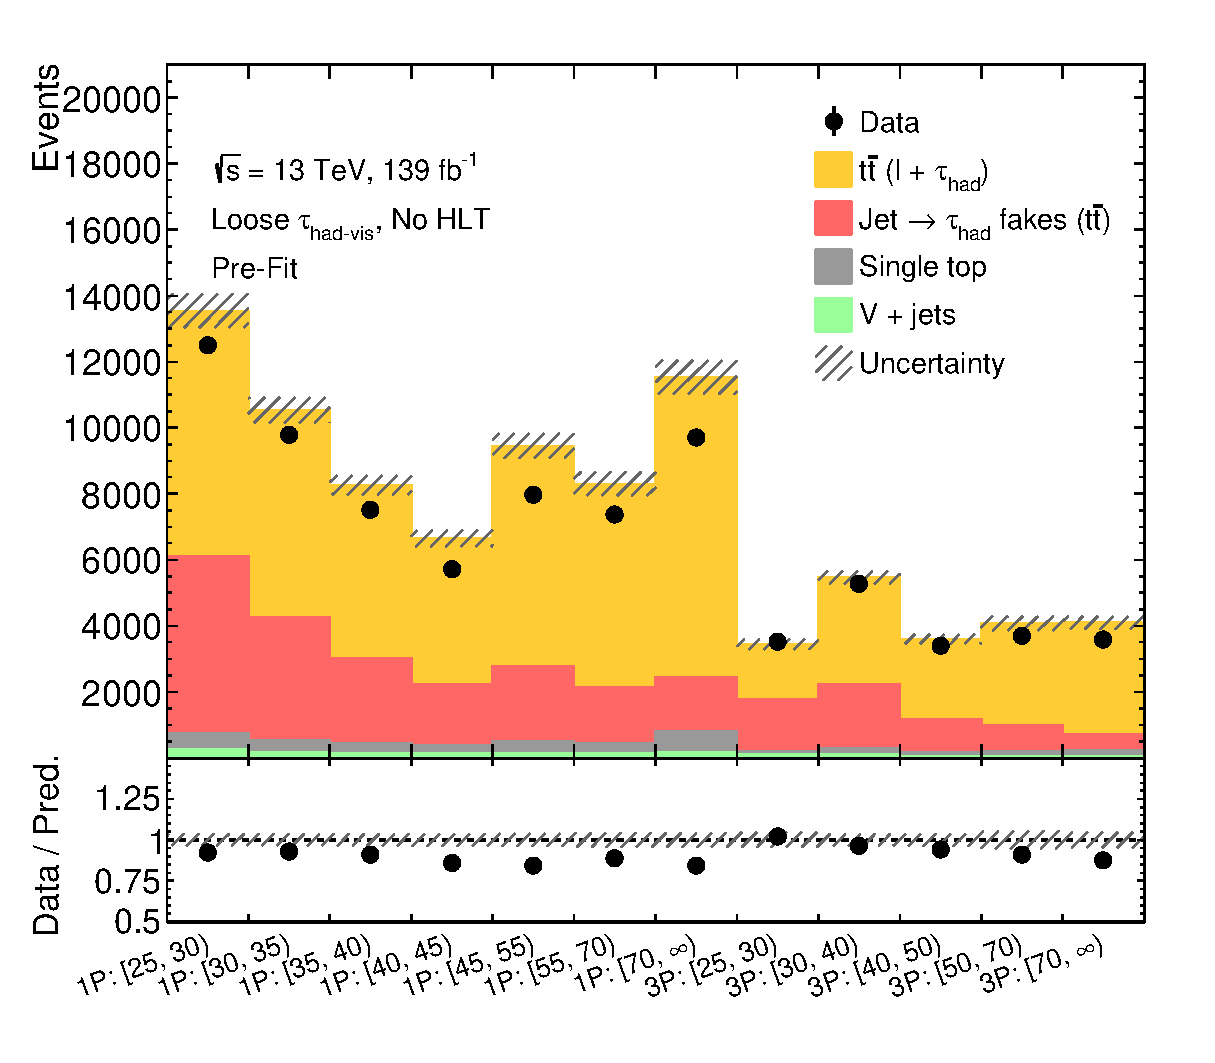
\includegraphics[width=\textwidth]{ttbarSF/Summary_offl}

    \caption{Events without trigger-level \tauid requirements.}
  \end{subfigure}\hfill%
  \begin{subfigure}[t]{.48\textwidth}
    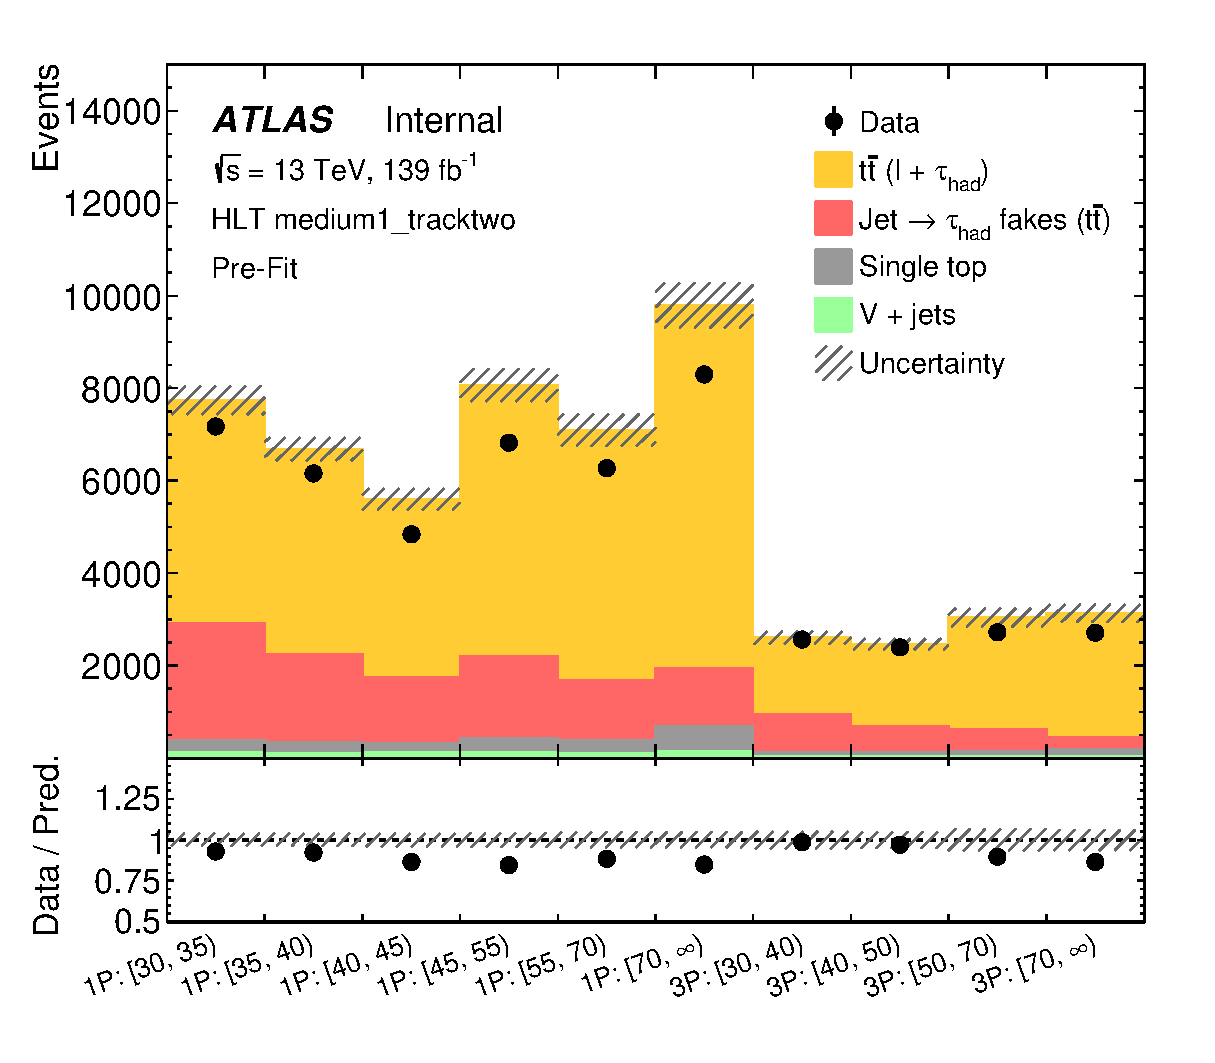
\includegraphics[width=\textwidth]{ttbarSF/Summary_tau25}

    \caption{Events passing \tauhadvis trigger-matching and the
      \texttt{HLT\_tau25\_medium1\_tracktwo} trigger.}
  \end{subfigure}

  \caption[Expected and observed event yields in regions of \tauhadvis candidate
  \Ntracks and \pT in the SF-CR.]{Expected and observed event yields in regions
    of \tauhadvis candidate \Ntracks and \pT in the SF-CR. The bins are labelled
    as ``1P'' and ``3P'' for $\Ntracks = 1$ and $\Ntracks = 3$, respectively,
    and the \pT intervals are given in units of \si{\GeV}. The background model
    is shown prior to the fit.}%
  \label{fig:ttbarsf_region_summary_prefit}
\end{figure}

A discriminant is required to distinguish between \ttbar with and without
\faketauhadvis since only the former is sensitive to \jettotauhadvis
misidentification efficiencies. The transverse mass of the electron/muon and
\pTmissAbs is used for this purpose, which is defined as
\begin{align*}
  \mTW = \sqrt{2 | \myvec{p}_{\text{T}}^{\ell} | | \pTmiss | \left( 1 - \cos \Delta\phi \right)} \,\text{,}
\end{align*}
where $\Delta \phi$ is the angle between the lepton transverse momentum,
$\myvec{p}_{\text{T}}^{\ell}$, and the missing transverse momentum, \pTmiss. The
\mTW discriminant targets the differences between di- and semi-leptonic decay
modes of \ttbar that are the primary sources of events with true- and
\faketauhadvis, respectively. The differences are illustrated
in~\Cref{fig:ttbarsf_mtw_pdf}, with di-leptonic decay modes of \ttbar showing a
heavy tail towards large \mTW due to the presence of additional neutrinos, while
semi-leptonic decay modes have a more pronounced peak close to the mass of the
$W$~boson.


\begin{figure}[htbp]
  \centering

  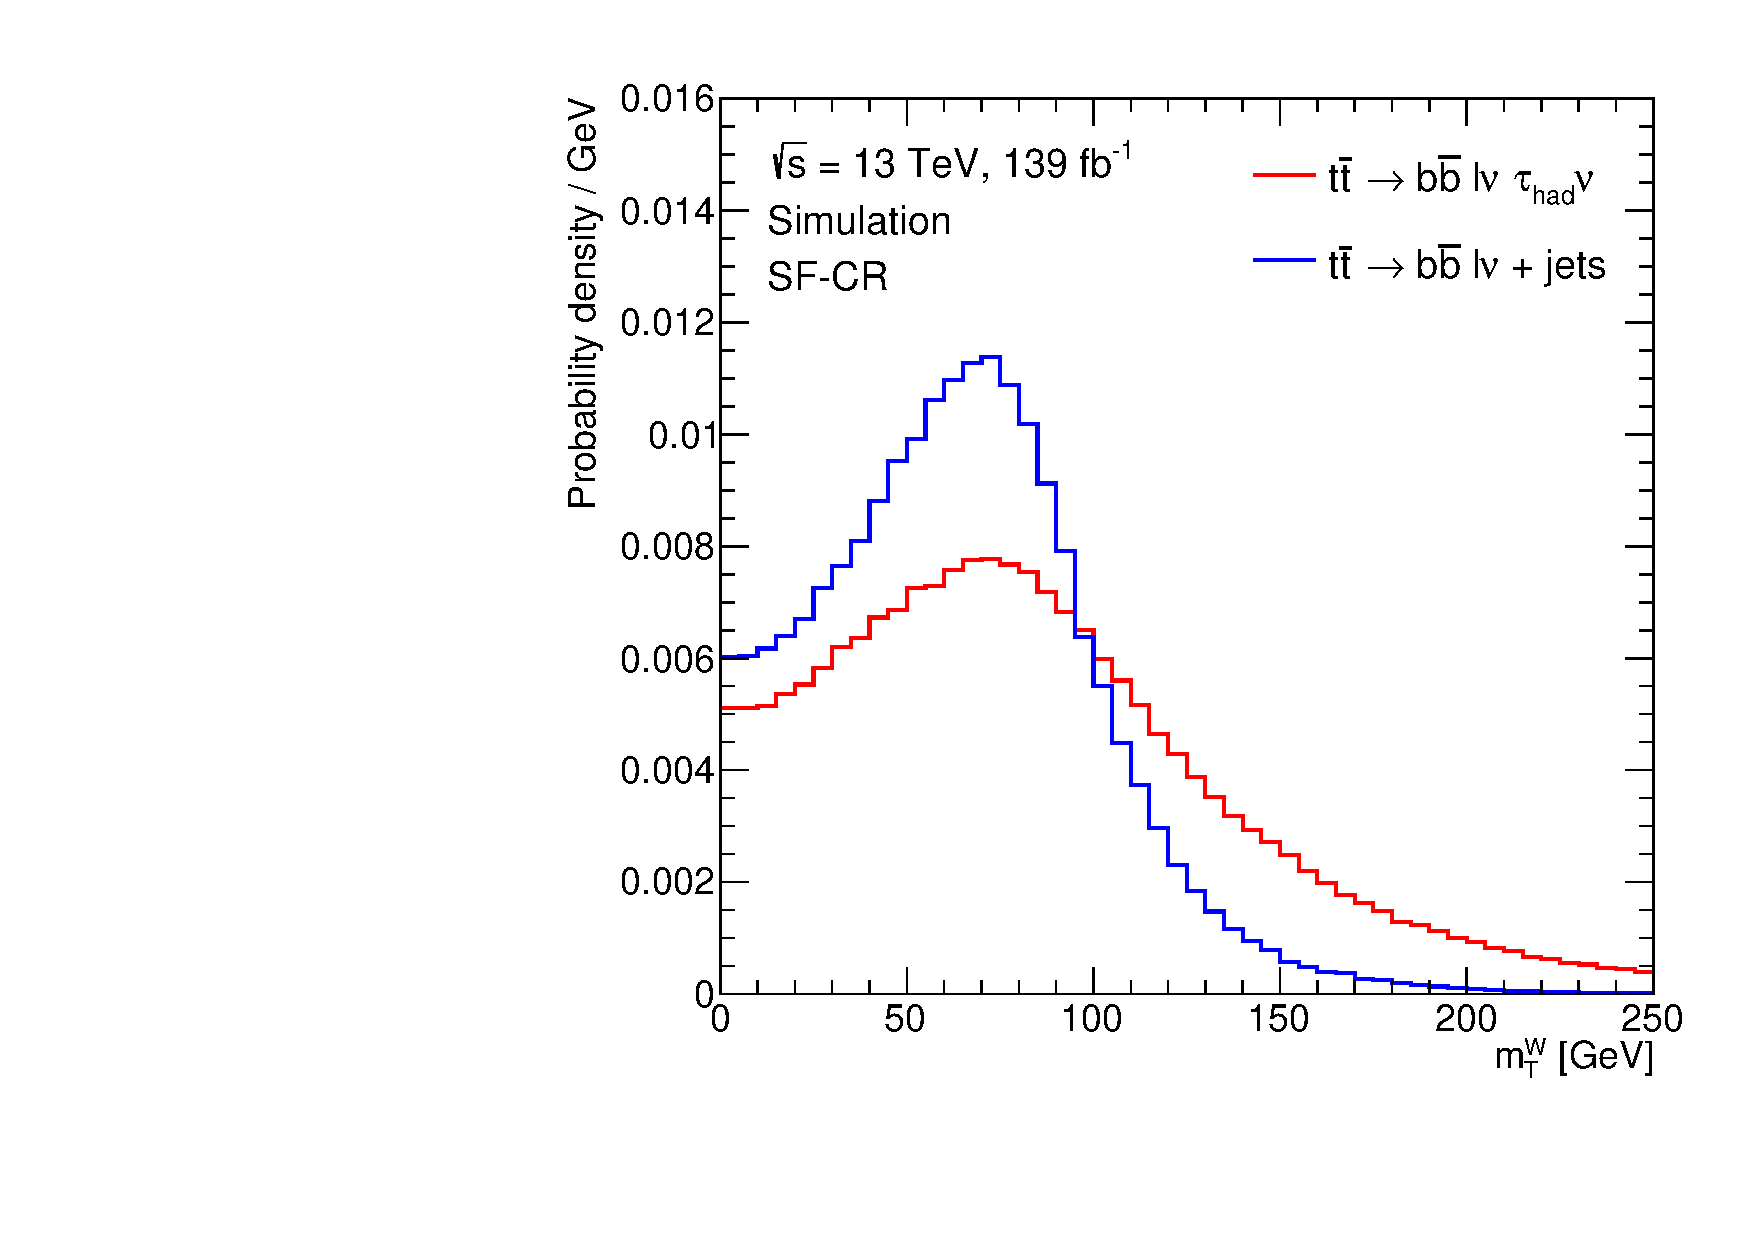
\includegraphics[width=0.45\textwidth, trim=0.5cm 1.5cm 0.3cm 0.3cm,
  clip]{ttbarSF/mtw_pdf}

  \caption[Distribution of the transverse mass of the lepton and \pTmiss for
  simulated \ttbar events in the SF-CR.]{Distribution of the transverse mass of
    the lepton and \pTmiss for simulated \ttbar events in the SF-CR. The
    distributions are inclusive in \pT and \Ntracks of the \tauhadvis
    candidate.}%
  \label{fig:ttbarsf_mtw_pdf}
\end{figure}

The \faketauhadvis SFs are measured using a simultaneous likelihood fit of the
binned \mTW distributions in all regions of \tauhadvis candidate \pT and
\Ntracks. The fit model is constructed using simulated \ttbar, single-top, and
\Vjets events. The sample of \ttbar events is split by whether the reconstructed
\tauhadvis candidate is a \faketauhadvis or not. The overall normalisation of
the \ttbar background, irrespective of whether events contain a \faketauhadvis,
is free to vary in the model.  In every region of \tauhadvis candidate
\Ntracks and \pT, an unconstrained SF is introduced that changes the
normalisation of the \ttbarFakes background in this region. These \faketauhadvis
SFs are considered as the POIs of the measurement.

The pre-fit expectation of the model in two exemplary regions is shown
in~\Cref{fig:ttbarsf_mtw_examples_prefit} for SF-CR events passing the
\verb|HLT_tau25_medium1_tracktwo| trigger and trigger-matching. The binning of
the \mTW discriminants is the same in all \tauhadvis candidate \pT and \Ntracks
regions.

\begin{figure}[htbp]
  \centering

  \begin{subfigure}{.48\textwidth}
    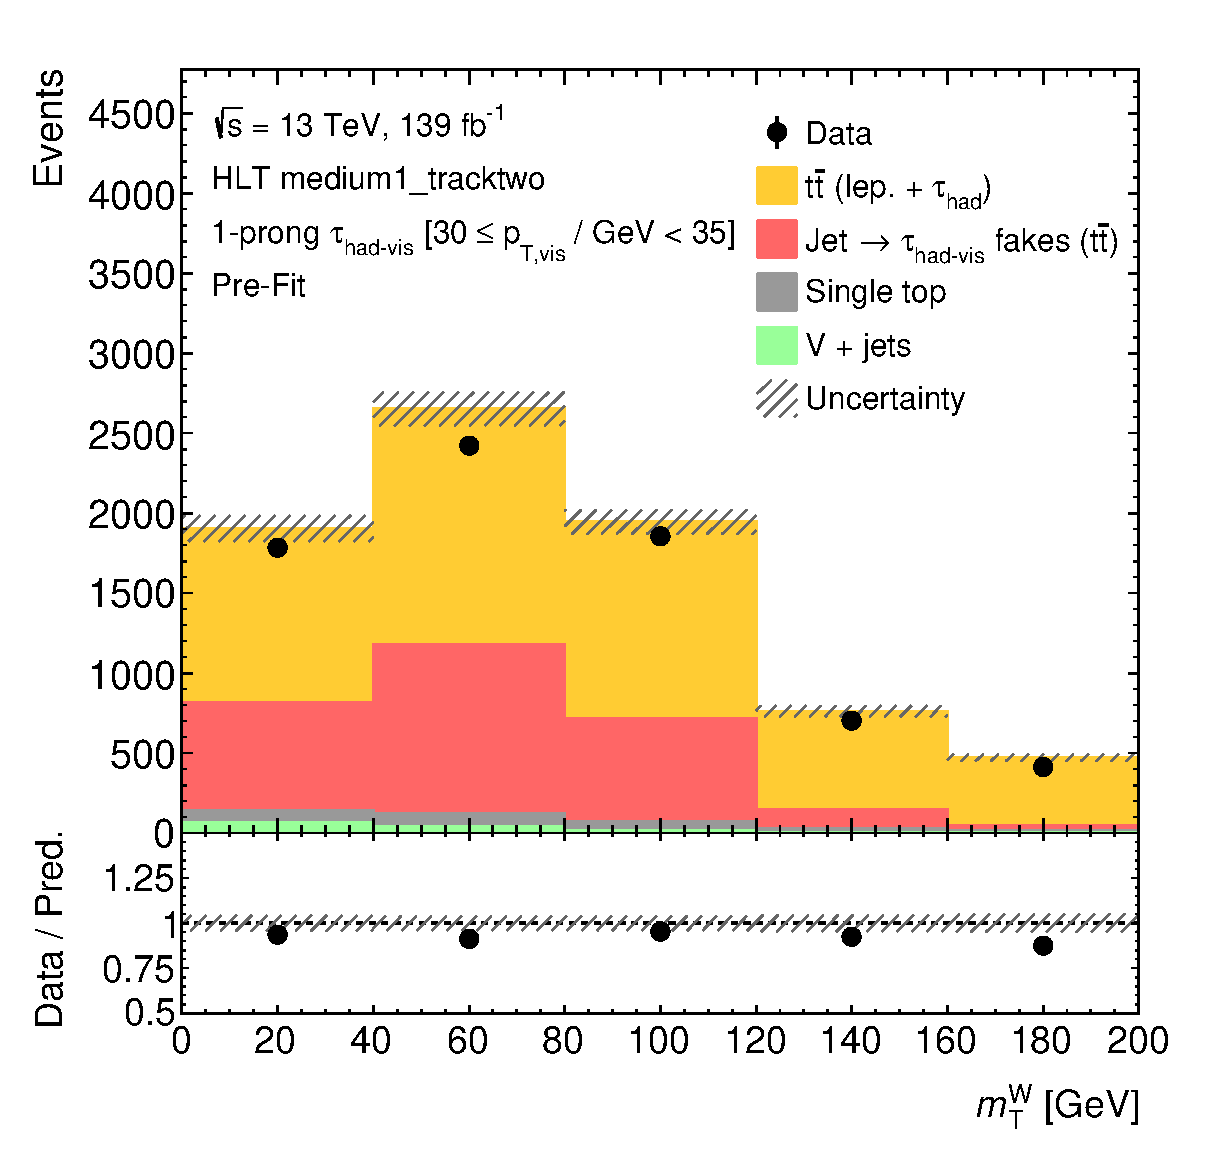
\includegraphics[width=\textwidth]{ttbarSF/tau25/TauPt3035_1P}
    \caption{$\Ntracks = 1$ and $\SI{30}{\GeV} \leq \pT < \SI{35}{\GeV}$.}
  \end{subfigure}\hfill%
  \begin{subfigure}{.48\textwidth}
    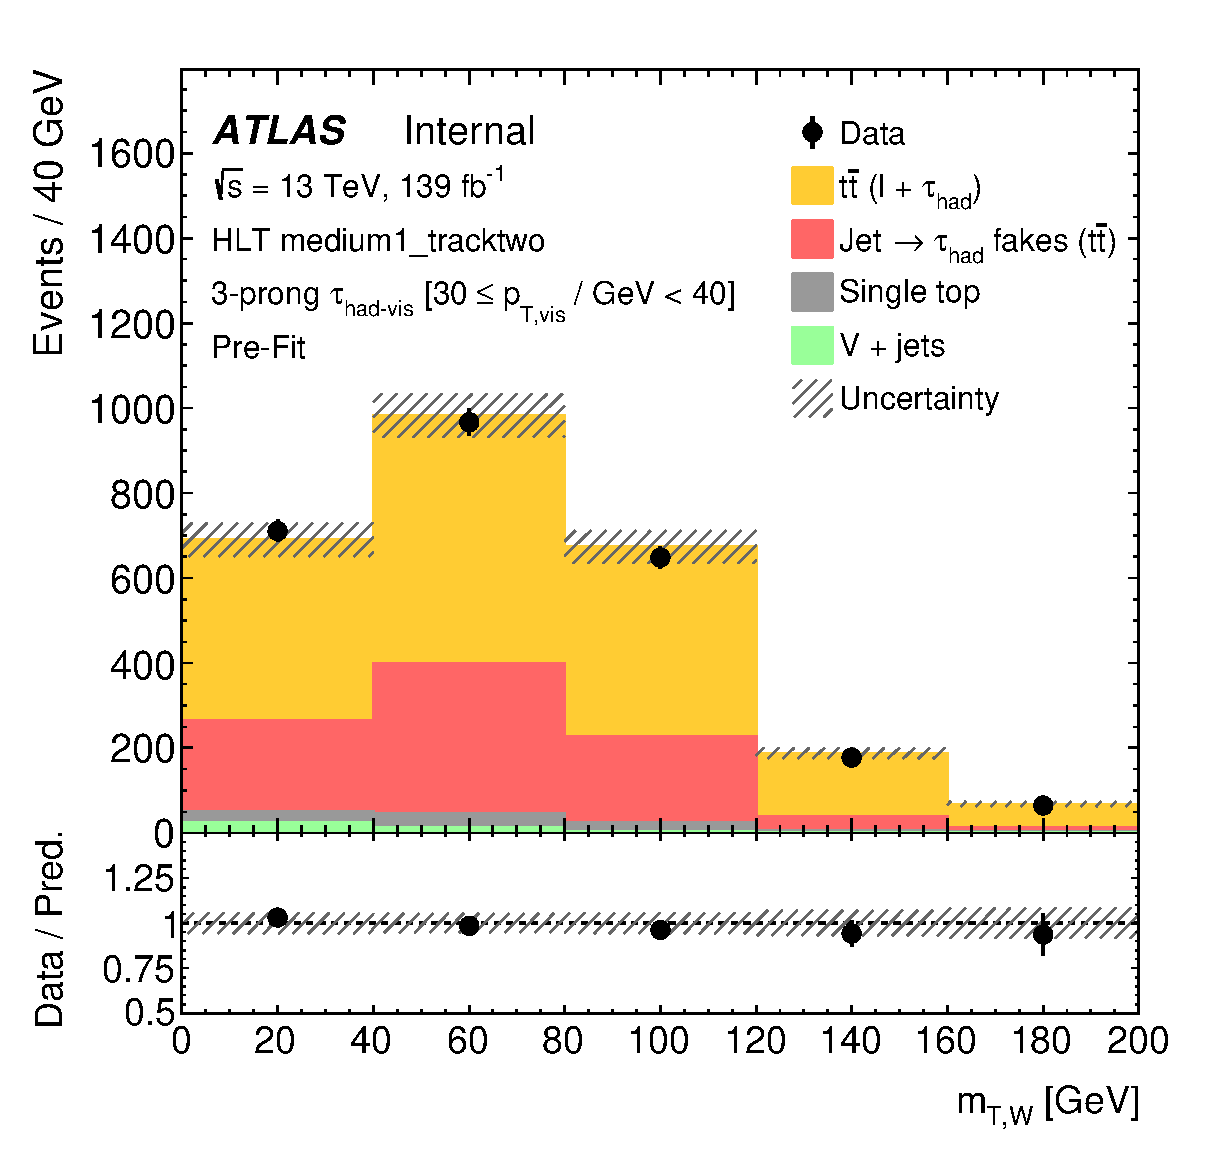
\includegraphics[width=\textwidth]{ttbarSF/tau25/TauPt3040_3P}
    \caption{$\Ntracks = 3$ and $\SI{30}{\GeV} \leq \pT < \SI{40}{\GeV}$.}
  \end{subfigure}

  \caption[Pre-fit \mTW distribution in two exemplary regions of the SF
  measurement.]{Pre-fit \mTW distribution in two exemplary \tauhadvis candidate
    \Ntracks and \pT regions of the SF measurement after requiring events to
    pass the \texttt{HLT\_tau25\_medium1\_tracktwo} trigger and
    trigger-matching. Events with $\mTW > \SI{200}{\GeV}$ are included in the
    last bin of the histograms.}%
  \label{fig:ttbarsf_mtw_examples_prefit}
\end{figure}


\subsubsection{Uncertainties in the Scale Factor Measurement}

Several experimental and theoretical uncertainties are considered in the SF
measurement. In general, these uncertainties can affect the normalisation and
shape of the expected \mTW distribution for a given process in all regions
entering the fit. The uncertainties included in the SF measurement and their
treatment closely follows the approach taken in
\Cref{sec:uncertainties,sec:statistical_analysis} to interpret the results of
the search for Higgs boson pair production. Therefore, the uncertainties
included in the SF measurement are only briefly summarised.

Experimental uncertainties affecting the reconstruction and selection
efficiencies of electrons, muons, \tauhadvis, and jets are accounted for in the
SF measurement, including uncertainties on the efficiencies of
$b$-tagging. Uncertainties on the reconstructed \pTmissAbs are propagated to the
\mTW distributions in all regions. Trigger efficiency uncertainties are
considered for single-lepton and single-\tauhadvis
triggers.\footnote{Uncertainties on single-\tauhadvis trigger efficiencies are
  only considered for SF measurements taking into account trigger-level \tauid
  requirements.}  Uncertainties on the re-weighting of the pile-up conditions in
simulation and the integrated luminosity used to normalise simulated event
samples are included in the measurement as well. Lastly, statistical
uncertainties from the finite size of the simulation samples are included
according to the simplified Barlow--Beeston method~\cite{barlow1993,conway2011}.

Theory uncertainties on the modelling of \ttbar production using simulation are
derived for this measurement according to prescriptions developed by the ATLAS
collaboration, which are summarised in \Cref{app:top_uncertainties}. An
uncertainty on the simulation of the hard interaction and matching to the parton
shower is derived by comparison with an alternative matrix element generator and
matching scheme. Uncertainties on the modelling of the parton shower,
hadronisation, and underlying event are determined by comparison with an
alternative parton shower program. The effect of missing higher orders in the
truncated perturbative expansion in \alphas is probed by performing variations
of renormalisation and factorisation scales. Finally, uncertainties on the
modelling of additional emissions are derived by performing variations of the
simulated initial- and final-state radiation. Modelling uncertainties are
derived separately for \ttbar events with and without \faketauhadvis, but are
regarded as correlated in the fit model if they originate from the same
source. Effects of the \ttbar modelling uncertainties on the shape of the \mTW
discriminants and the expected number of events in different \tauhadvis
candidate \Ntracks and \pT regions are considered in the fit model.

Reduced sets of theory uncertainties are considered for minor backgrounds in the
SF measurement. Uncertainties on the cross sections of single-top and \Vjets
production are included in the model. Due to the known normalisation discrepancy
of \Vjets production in the presence of jets originating from heavy flavour
quarks, an additional normalisation uncertainty of \SI{30}{\percent} is assigned
to the \Vjets background.


\subsubsection{Results of the Scale Factor Measurement}

The measured \faketauhadvis SFs are shown in \Cref{fig:ttbarSF_postfit_SF}.
% for all relevant \tauid criteria.
The size of the corrections described by the SFs can reach up to
\SI{55}{\percent} for \faketauhadvis of high \pT, where simulation overestimates
the contribution of \faketauhadvis in \ttbar. SFs for \faketauhadvis
reconstructed as 1-prong (3-prong) candidates with $\pT < \SI{70}{\GeV}$ are
within \SI{20}{\percent} (\SI{40}{\percent}) of unity. Only small differences
are observed between SFs measured for different \tauid requirements at
trigger-level, as is shown
in~\Cref{fig:ttbarSF_postfit_SF_c,fig:ttbarSF_postfit_SF_d}.

\begin{figure}[htbp]
  \centering

  \begin{subfigure}[t]{.495\textwidth}
    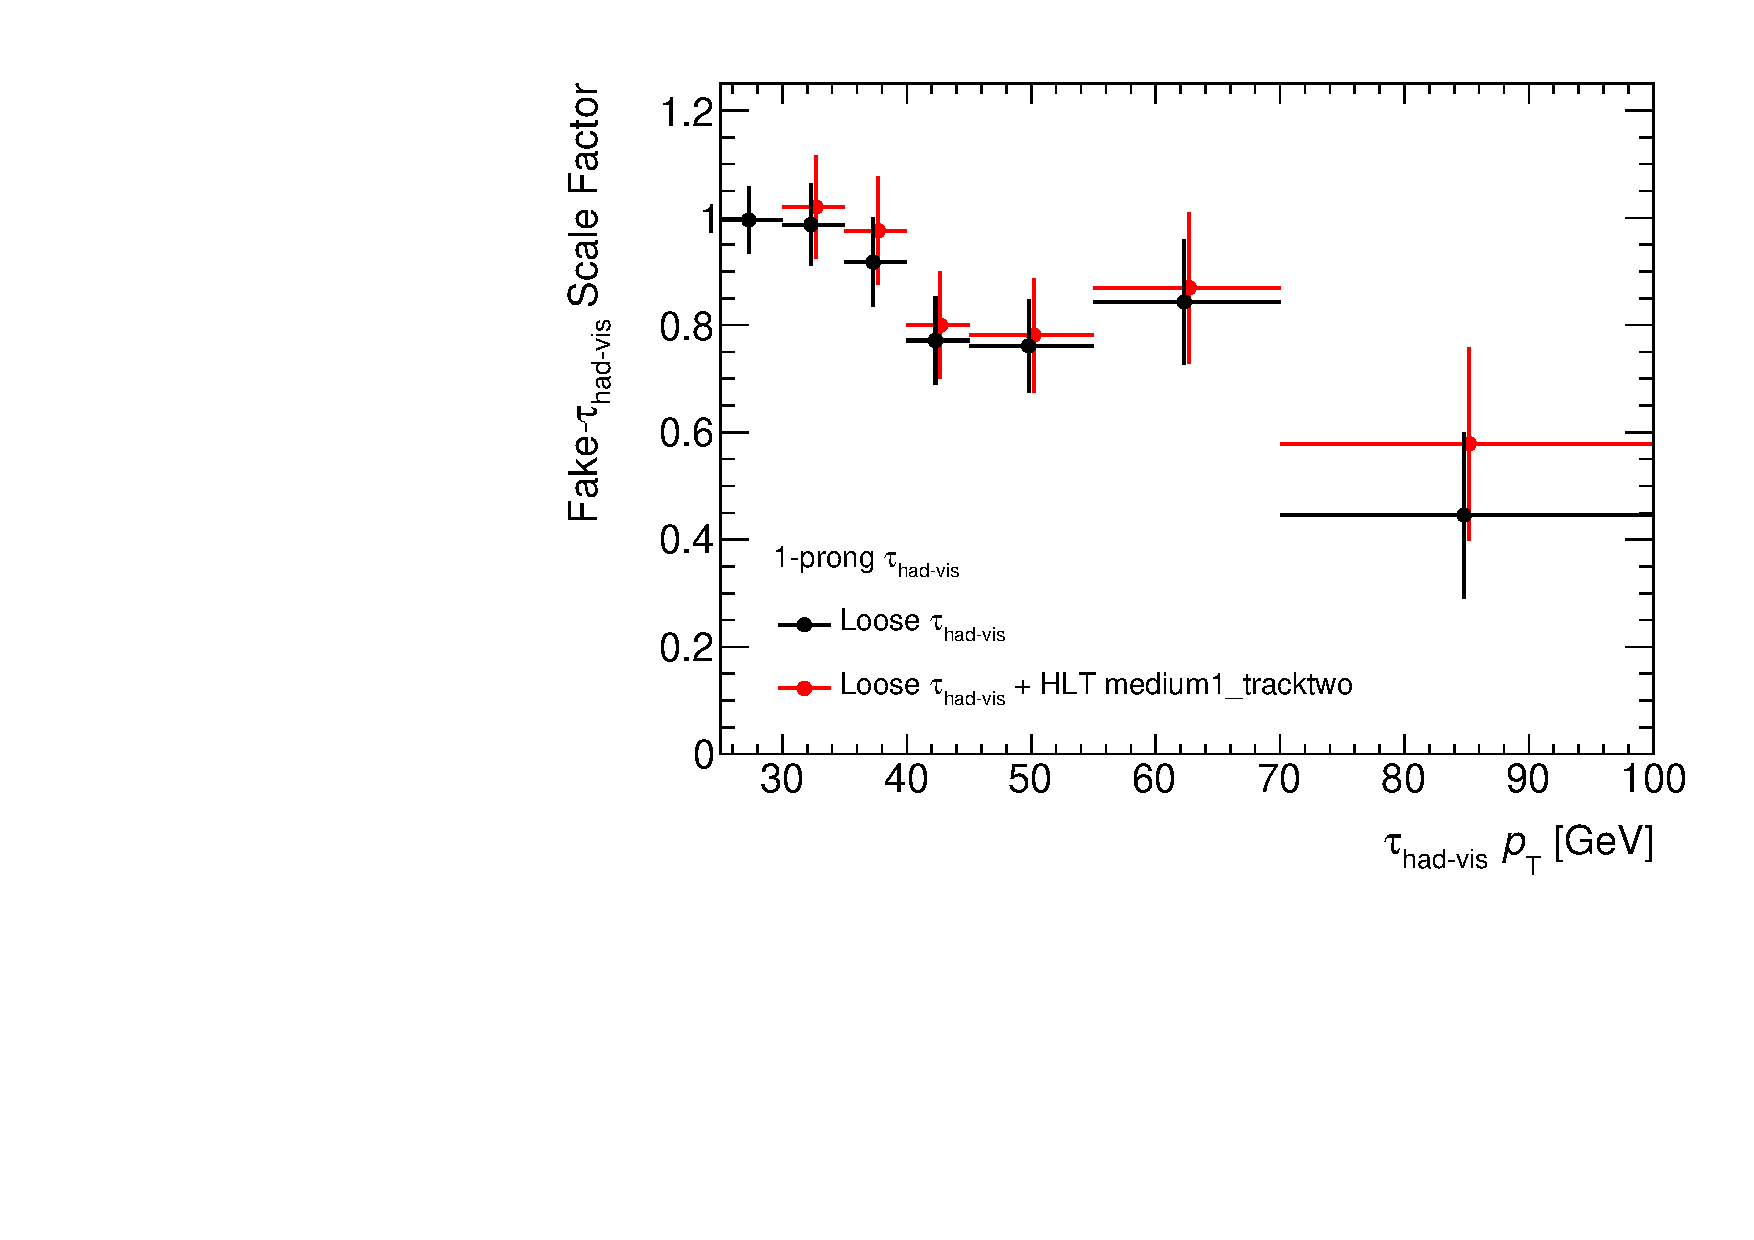
\includegraphics[width=\textwidth]{ttbarSF/ttbarSF_offl_tau25_1p}
    \caption{}
    \label{fig:ttbarSF_postfit_SF_a}
  \end{subfigure}\hfill%
  \begin{subfigure}[t]{.495\textwidth}
    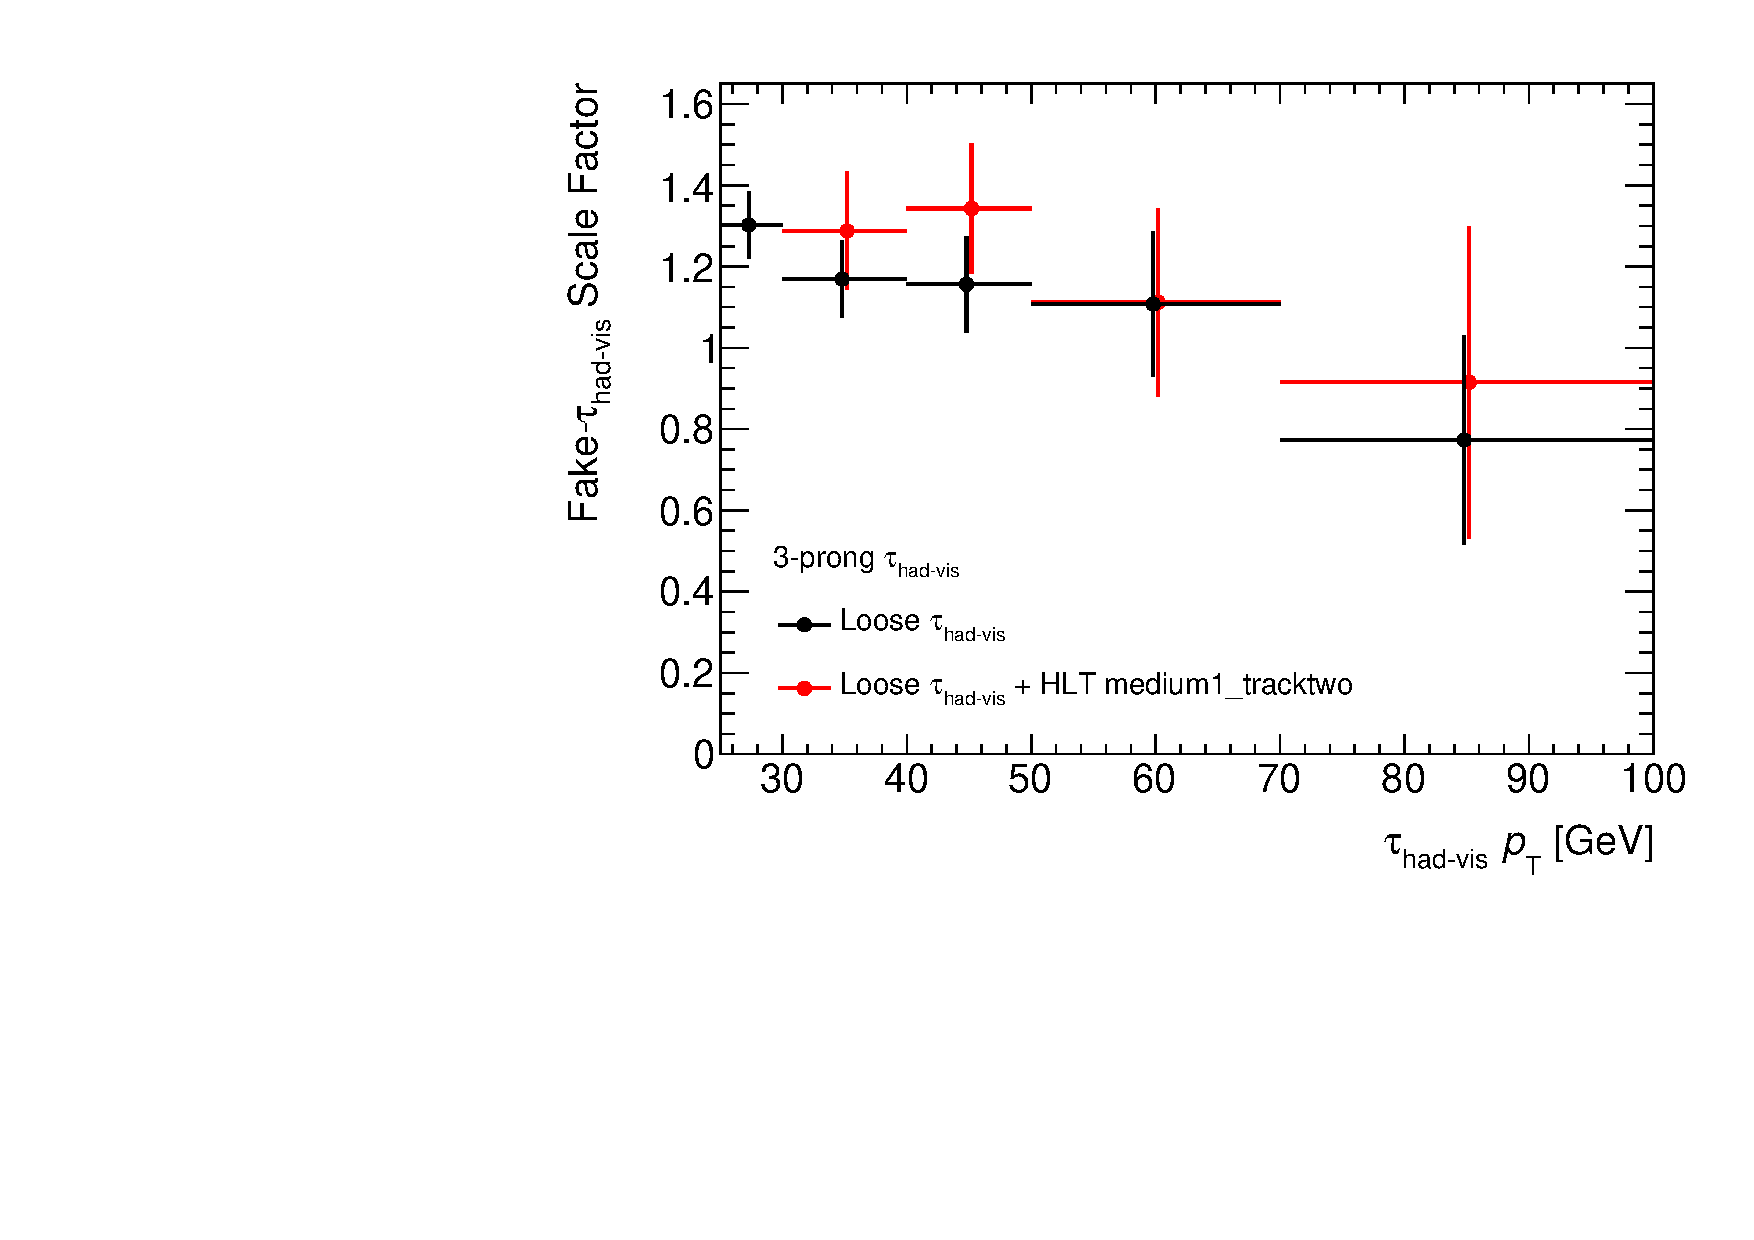
\includegraphics[width=\textwidth]{ttbarSF/ttbarSF_offl_tau25_3p}
    \caption{}
    \label{fig:ttbarSF_postfit_SF_b}
  \end{subfigure}

  \begin{subfigure}[t]{.495\textwidth}
    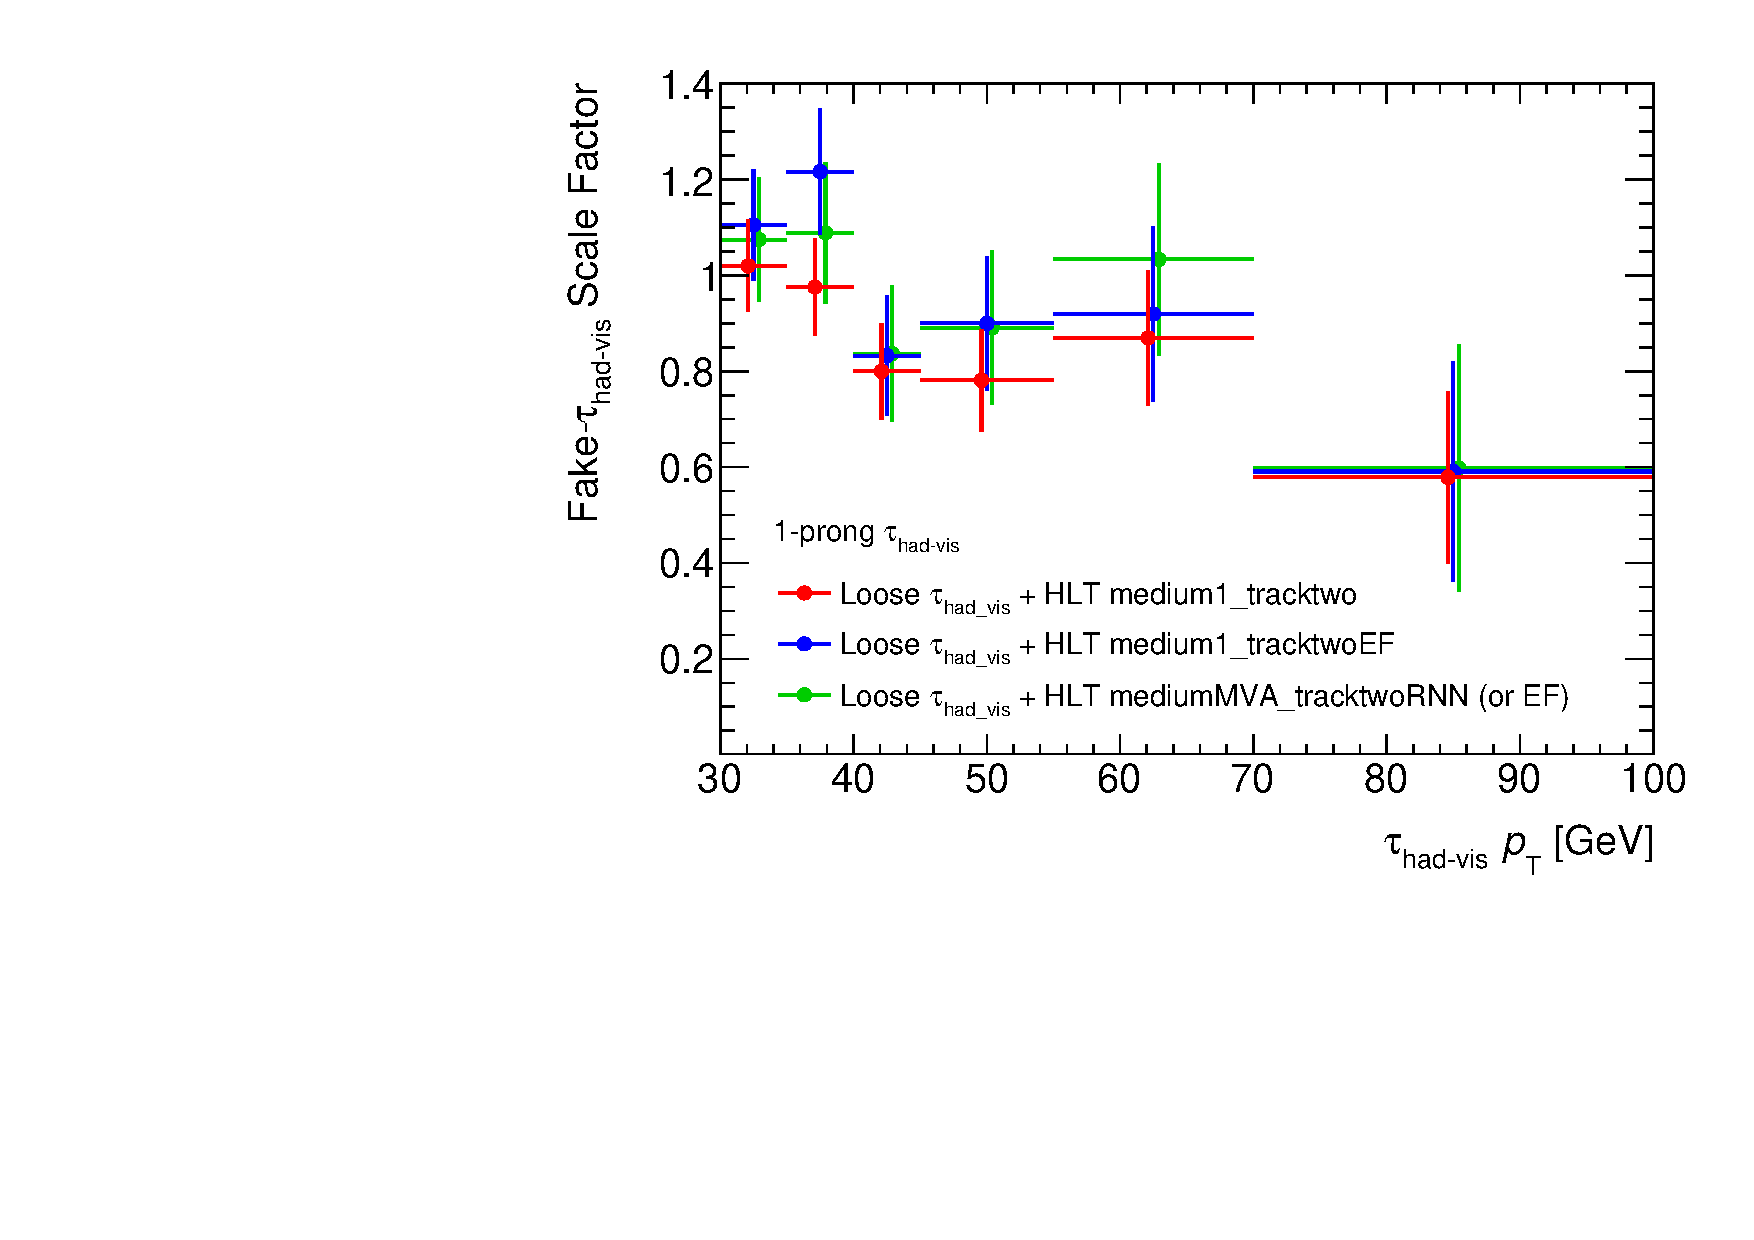
\includegraphics[width=\textwidth]{ttbarSF/ttbarSF_tau25_1p}
    \caption{}
    \label{fig:ttbarSF_postfit_SF_c}
  \end{subfigure}\hfill%
  \begin{subfigure}[t]{.495\textwidth}
    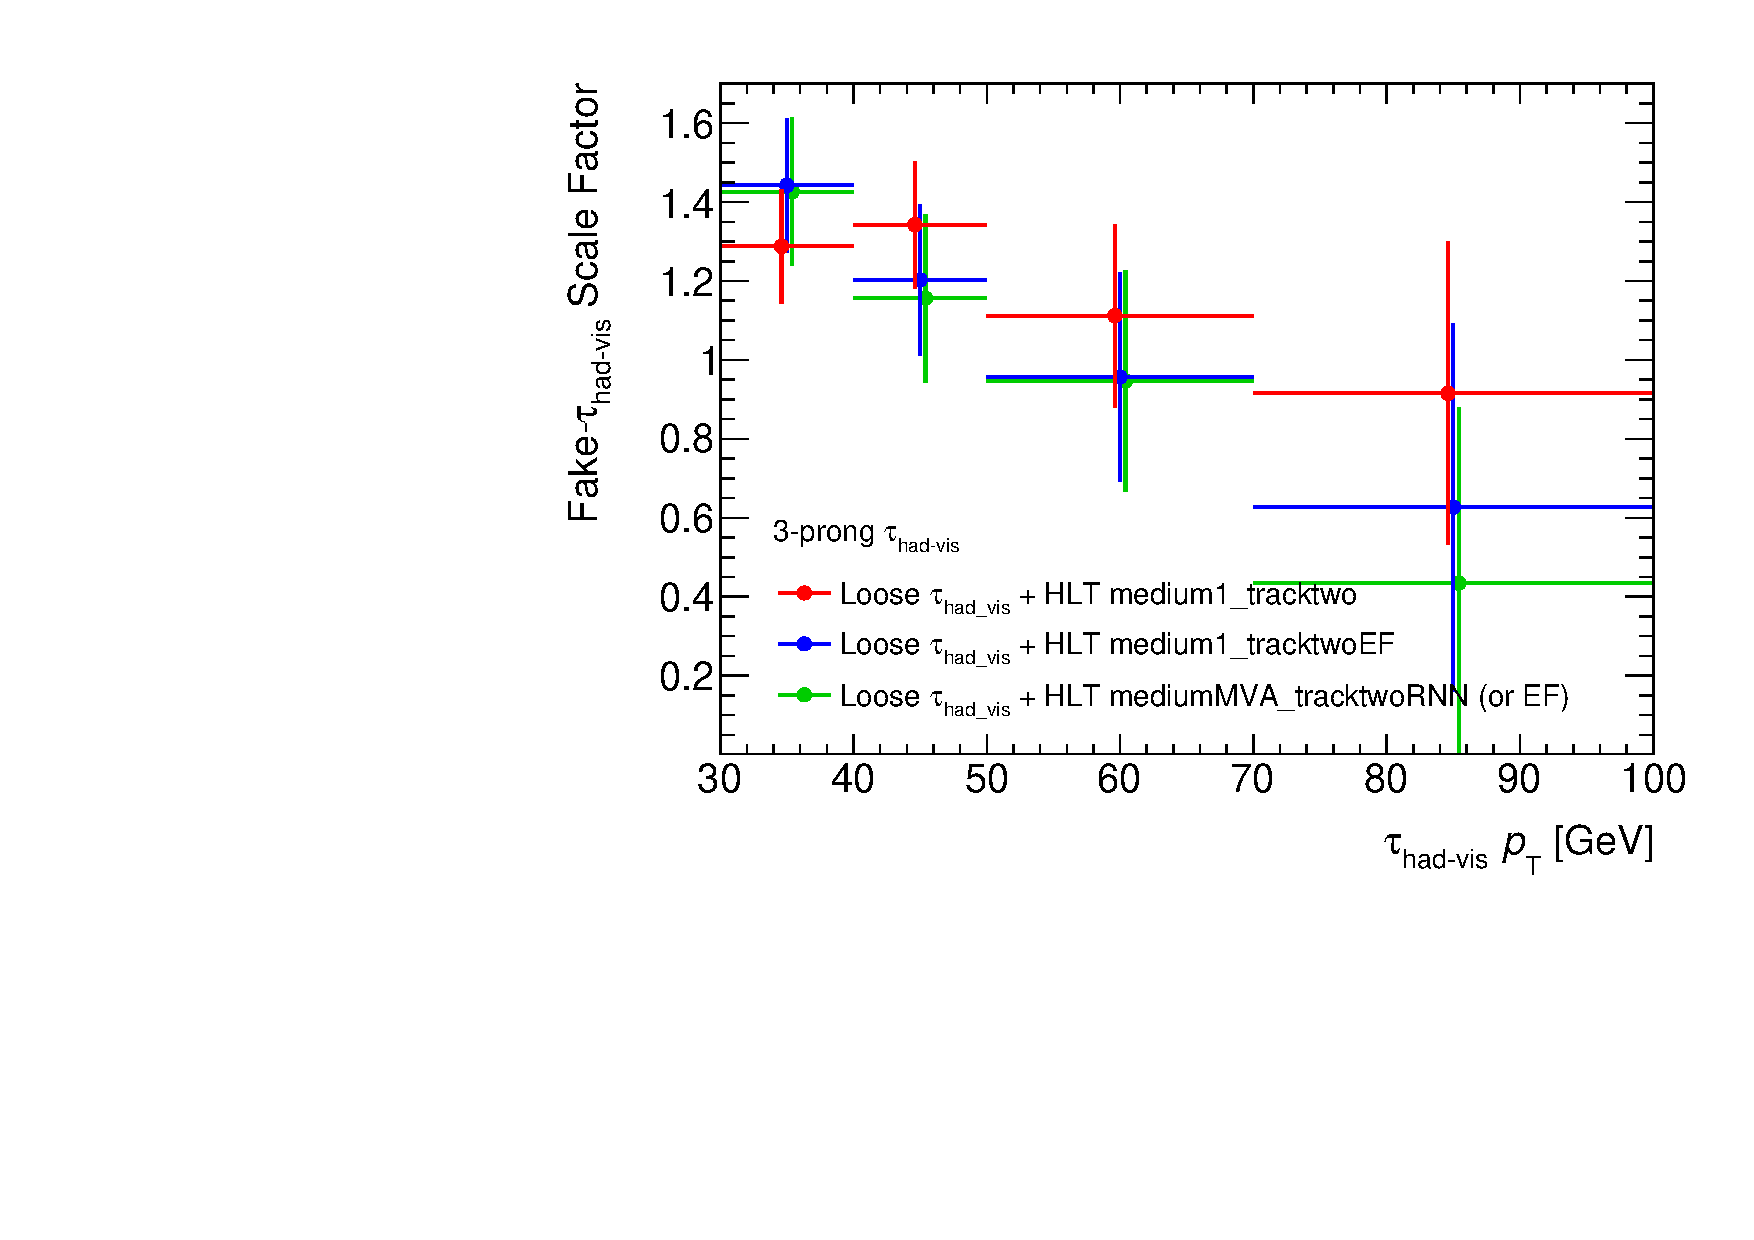
\includegraphics[width=\textwidth]{ttbarSF/ttbarSF_tau25_3p}
    \caption{}
    \label{fig:ttbarSF_postfit_SF_d}
  \end{subfigure}

  \caption[\Faketauhadvis SFs for different \tauid criteria.]{\Faketauhadvis SFs
    for different \tauid criteria. Figures~(a) and (b) compare the SFs with and
    without tau identification at the HLT. The effect of different
    \tauhadvis-triggers on the extracted SFs is shown in Figures~(c) and (d). In
    all cases, the last bin summarises the SFs for \tauhadvis candidates with
    $\pT \geq \SI{70}{\GeV}$. The markers are shifted from their geometrical bin
    centres for illustration purposes only.}%
  \label{fig:ttbarSF_postfit_SF}
\end{figure}

The fit model and the corresponding fit results are checked by comparing the
post-fit predictions of the model with the observed data in all \tauhadvis
candidate \Ntracks and \pT regions. In addition, pulls and constraints of NPs as
well as correlations between NPs and the POIs are inspected. Exemplary post-fit
predictions of the model are shown in \Cref{fig:ttbarSF_postfit_ptmtw} in terms
of the \pT of \tauhadvis candidates and \mTW in the SF-CR after requiring events
to pass the \texttt{HLT\_tau25\_medium1\_tracktwo} trigger and trigger-matching.

\begin{figure}[htbp]
  \centering

  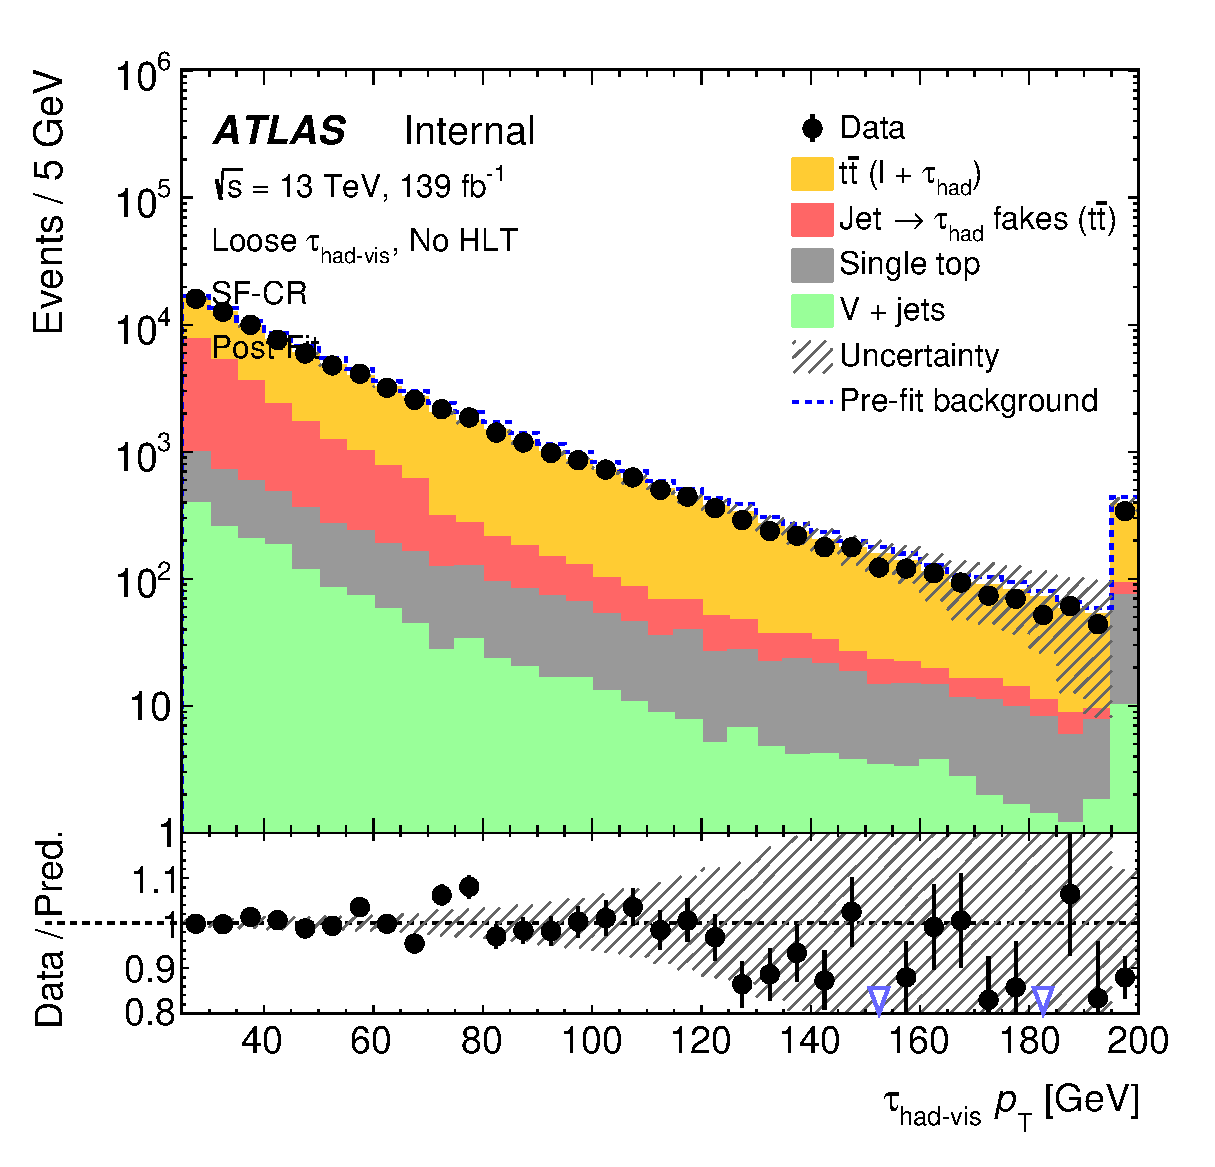
\includegraphics[width=0.49\textwidth]{ttbarSF/postfit_sfcr/PTVR_postFit}
  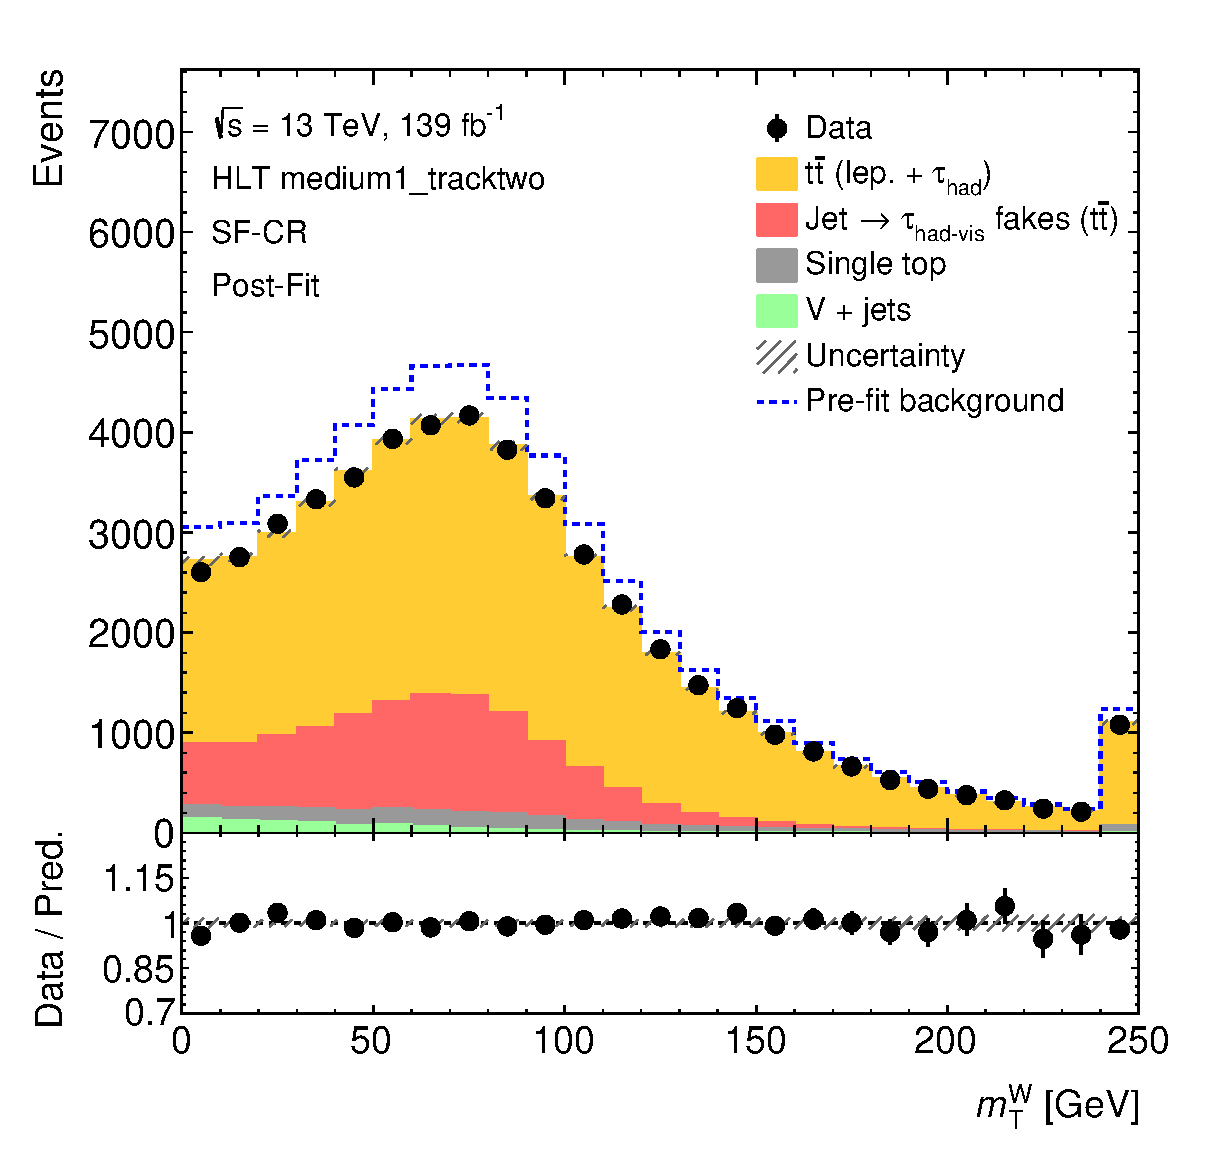
\includegraphics[width=0.49\textwidth]{ttbarSF/postfit_sfcr/MTWVR_postFit}

  \caption[Post-fit distributions of \tauhadvis candidate \pT and \mTW in the
  SF-CR.]{Post-fit distributions of \tauhadvis candidate \pT and \mTW in the
    SF-CR for events passing the \texttt{HLT\_tau25\_medium1\_tracktwo} trigger
    and trigger-matching. Both distributions are inclusive in \Ntracks and \pT
    of \tauhadvis candidates. Events with \tauhadvis \pT (\mTW) larger than
    \SI{200}{\GeV} (\SI{250}{\GeV}) are included in the last bin. The
    uncertainty band contains all statistical and systematic uncertainties,
    including post-fit uncertainties on \faketauhadvis SFs and on the overall
    \ttbar normalisation factor.}%
  \label{fig:ttbarSF_postfit_ptmtw}
\end{figure}

The post- and pre-fit values of all NPs agree within their
uncertainties. Few instances are observed where the SF measurement puts more
stringent constraints on the values of NPs than expected from
the prior estimation of the associated uncertainty. These cases are the
\pTmissAbs scale uncertainty, the \ttbar modelling uncertainties resulting from
comparison with alternative ME/PS generators, and the \tauhadvis energy scale
uncertainty. The constraints on these parameters tend to be moderate with ratios
of post- to pre-fit uncertainties above \SI{70}{\percent}. Due to the
sensitivity of the \mTW discriminant to the modelling of \pTmissAbs and the
abundance of \ttbar events in the SF-CR, the fit is expected to have some power
to constrain the associated NPs. Moreover, the \tauhadvis energy
scale uncertainties are derived from $Z \ra \tau_{\mu} \tauhad$ tag-and-probe
measurements~\cite{ATLAS-CONF-2017-029}, which provide probe \tauhadvis with
smaller transverse momenta than the ones produced in \ttbar events. With the SF
measurement being performed in \Ntracks and \pT bins of the \tauhadvis candidate
and targeting \ttbar events, constraints on the \tauhadvis energy scale in the
SF measurement are expected.

% Pulls and constraints of nuisance parameters are examined for all scale factor
% measurements. The nuisance parameter estimates agree within uncertainties with
% the central values of their auxiliary measurements. Few instances are observed
% where the scale factor measurement puts more stringent constraints on nuisance
% parameters than expected from the prior estimation of the associated
% uncertainty. All constrained parameters have post-fit uncertainties larger
% than \SI{70}{\percent} with respect to the uncertainty prior to the fit,
% indicating only mild constraints.

% The largest nuisance parameter constraints, in the following given as the
% ratio of post- to pre-fit uncertainty, are observed for the \pTmissAbs scale
% uncertainty~(\SI{70}{\percent}), the ME / PS modelling uncertainties on
% \ttbar~(\SI{75}{\percent}), and \tauhadvis energy scale
% uncertainty~(\SI{80}{\percent}).  The \mTW discriminant is sensitive to the
% modelling of \pTmissAbs, thus some power to constrain nuisance parameters
% related to the modelling of \pTmissAbs in simulation is expected. Similarly,
% the SF-CR selects a large number of \ttbar events with high purity,
% consequently allowing to constrain the modelling uncertainties that are
% derived from two-sample comparisons. Finally, the measurements providing
% uncertainties on the \tauhadvis energy scale are performed in
% $Z \ra \tau_{\mu} \tauhad$ tag-and-probe~\cite{ATLAS-CONF-2017-029} which
% provides probe \tauhadvis with a softer transverse momentum spectrum compared
% to \tauhadvis produced in \ttbar events. With the binning of the measurement
% in \tauhadvis \pT, it is expected that the uncertainties on the \tauhadvis
% energy scale, particularly at high \tauhadvis~\pT, can be constrained by this
% measurement.

The limited discrimination power of \mTW in distinguishing \ttbar events with
and without \faketauhadvis leads to large anti-correlations between
\faketauhadvis SFs and the \ttbar normalisation factor. Due to this coupling,
positive correlations are induced between the SFs themselves. This is
illustrated in \Cref{fig:ttbarSF_corr_matrix} for an exemplary SF measurement.

% The fit model introduces large anti-correlations between the overall \ttbar
% normalisation and the extracted scale factors for \ttbar with \faketauhadvis. An
% exemplary correlation matrix for one measurement is shown
% in~\Cref{fig:ttbarSF_corr_matrix} showing the most relevant correlations between
% parameters of interest and nuisance parameters.  The anti-correlations are a
% result of the limited discrimination power of \mTW in distinguishing between
% \ttbar with true- and \faketauhadvis, which is especially poor for low
% \tauhadvis transverse momenta. Thus a change in the overall \ttbar
% normalisation, affecting both \ttbar with true and \faketauhadvis, can be
% partially compensated by an increase in the \faketauhadvis scale factors. This
% coupling between \faketauhadvis scale factors and \ttbar normalisation
% introduces large positive correlations also between the scale factors
% themselves.

\begin{figure}[htbp]
  \centering

  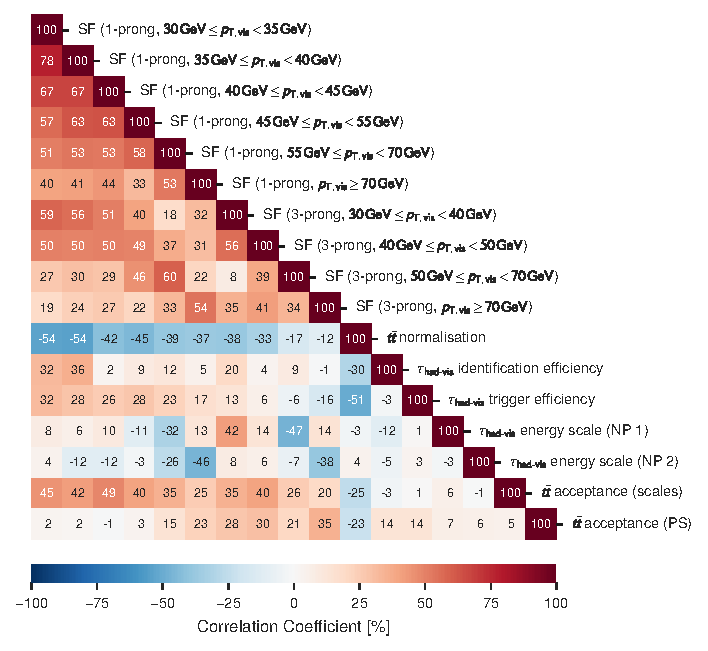
\includegraphics[scale=0.88]{ttbarSF/correlation_matrix}

  \caption[Post-fit correlation matrix between selected parameters of the
  \faketauhadvis SF measurement for the \texttt{HLT\_tau25\_medium1\_tracktwo}
  trigger.]{Post-fit correlation matrix between selected parameters of the
    \faketauhadvis SF measurement for the \texttt{HLT\_tau25\_medium1\_tracktwo}
    trigger. A reduced number of NPs is shown for illustration purposes. NPs are
    included if the absolute value of its correlation coefficient with at least
    one POI exceeds \SI{30}{\percent}.}%
  \label{fig:ttbarSF_corr_matrix}
\end{figure}

Correlations between the measured SFs need to be taken into account when
propagating the uncertainties on the SFs to the estimate of the \ttbarFakes
background in the \hadhad SR. This is achieved by providing a set of
decorrelated variations of the measurement that explains the total uncertainty
of all measured SFs. These variations can be used to propagate the uncertainties
to the background estimate without having to account for correlations.

A decorrelated set of variations is obtained by performing a linear
transformation of the $N$ measured SFs. The transformation is obtained by
diagonalising the post-fit SF covariance matrix, yielding a set of eigenvectors
and eigenvalues. The eigenvectors provide an alternative basis in which the
measurement is described by $N$~linear combinations of SFs with diagonal
covariance matrix. The eigenvalues correspond to the variance explained by
certain linear combinations of SFs.
% The covariance between two different linear combinations is
% zero by construction and the eigenvalues describe the variance of
% individual linear combinations.
In the frame with diagonal covariance matrix, the SF measurement is varied by
performing $\pm 1 \sigma$ variations, then transforming the resulting variations
back to the original, physically interpretable frame. This procedure yields $N$
systematic variations of the SF measurement, each with an up- and
down-variation. The variations are ordered by descending variance in the
diagonal frame, yielding variations that are roughly decreasing in their impact
on the total \ttbarFakes background estimate. An example of the results of the
decorrelation procedure is shown in~\Cref{fig:ttbarSF_eigenvariations}. The
effect of large correlations between SFs can be observed in the leading
variation (\texttt{EIGEN0}) as a systematic shift of the variation in all bins
with respect to the nominal result. In contrast, the variation explaining the
least variance (\texttt{EIGEN9}) only alters the SFs for 1-prong \faketauhadvis
with low transverse momenta.

\begin{figure}[htbp]
  \centering

  \begin{subfigure}[t]{.495\textwidth}
    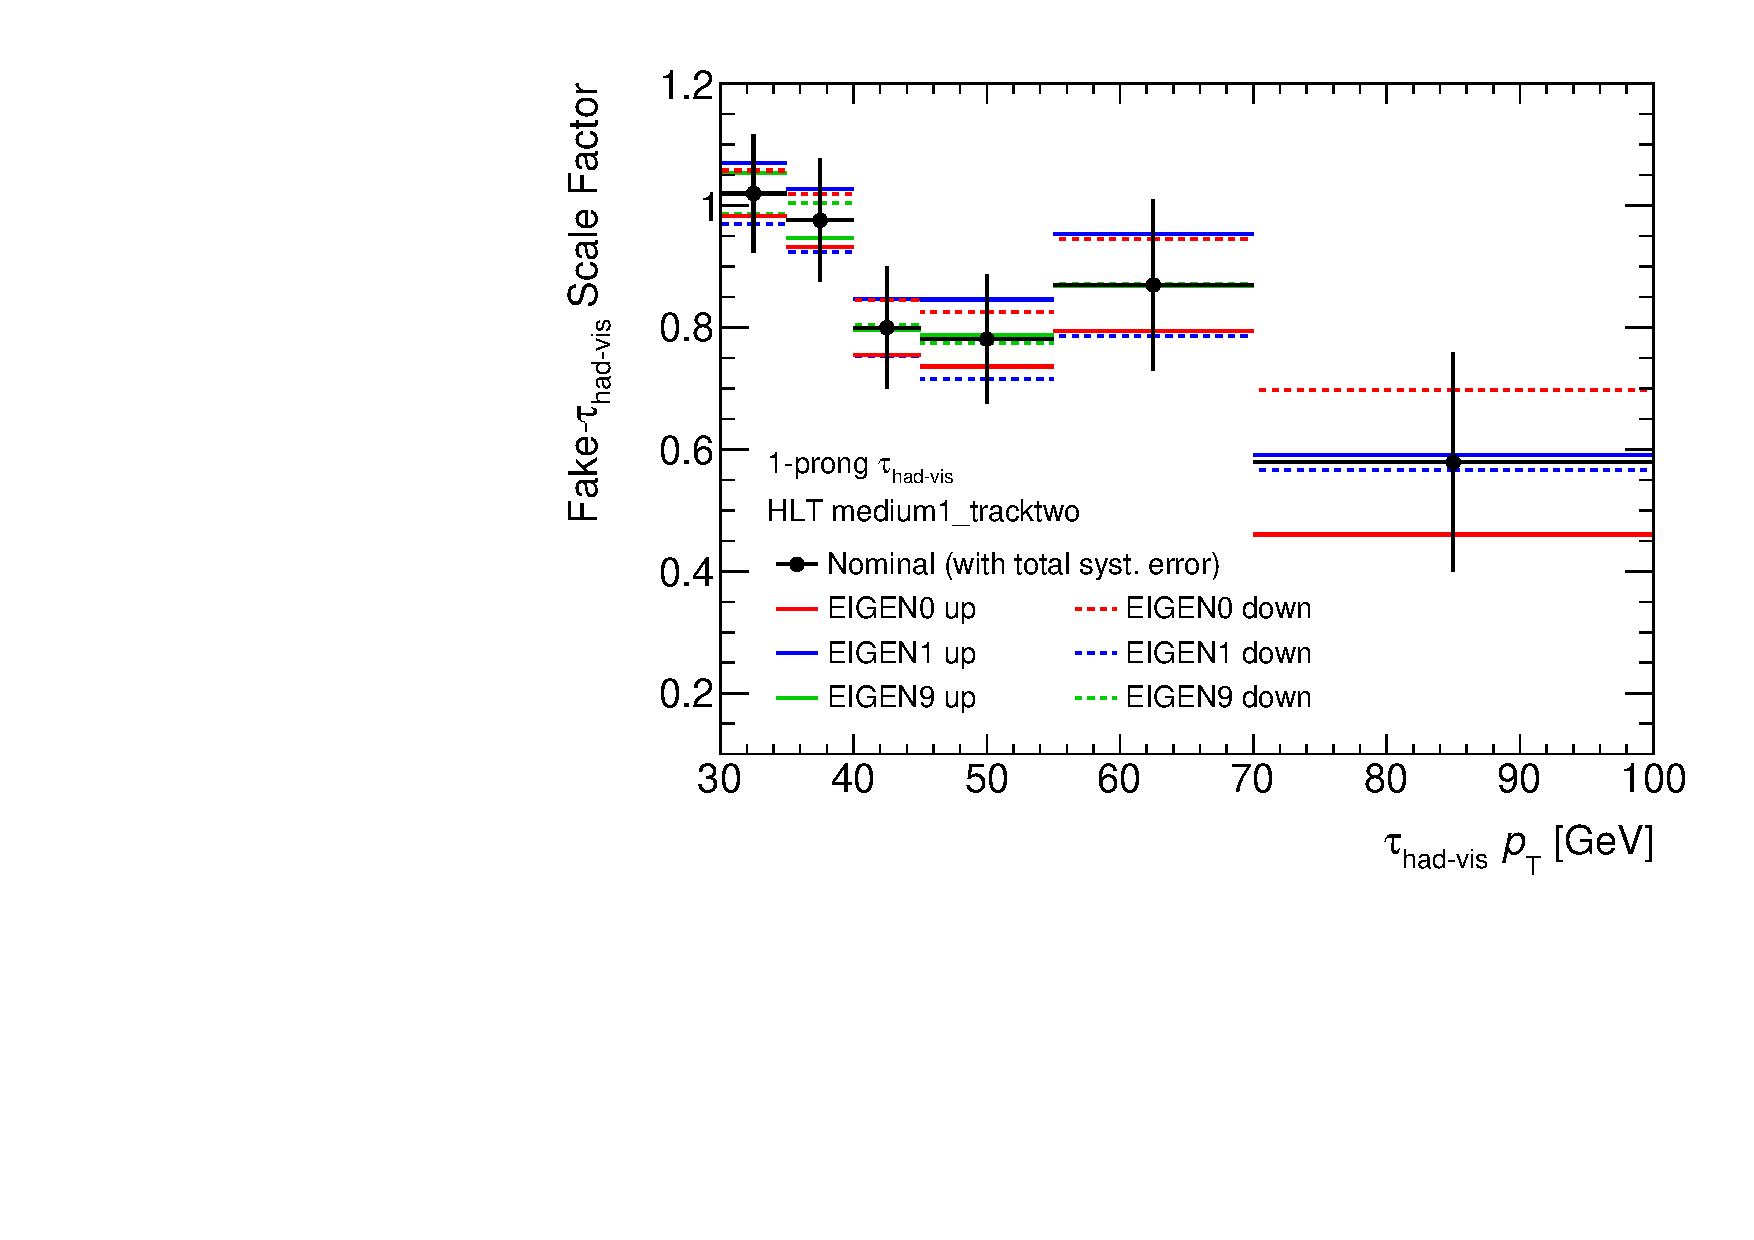
\includegraphics[width=\textwidth]{ttbarSF/ttbarSF_eigvar_1p}
    \caption{1-prong \tauhadvis}%
    \label{fig:ttbarSF_eigenvariations_1p}
  \end{subfigure}\hfill%
  \begin{subfigure}[t]{.495\textwidth}
    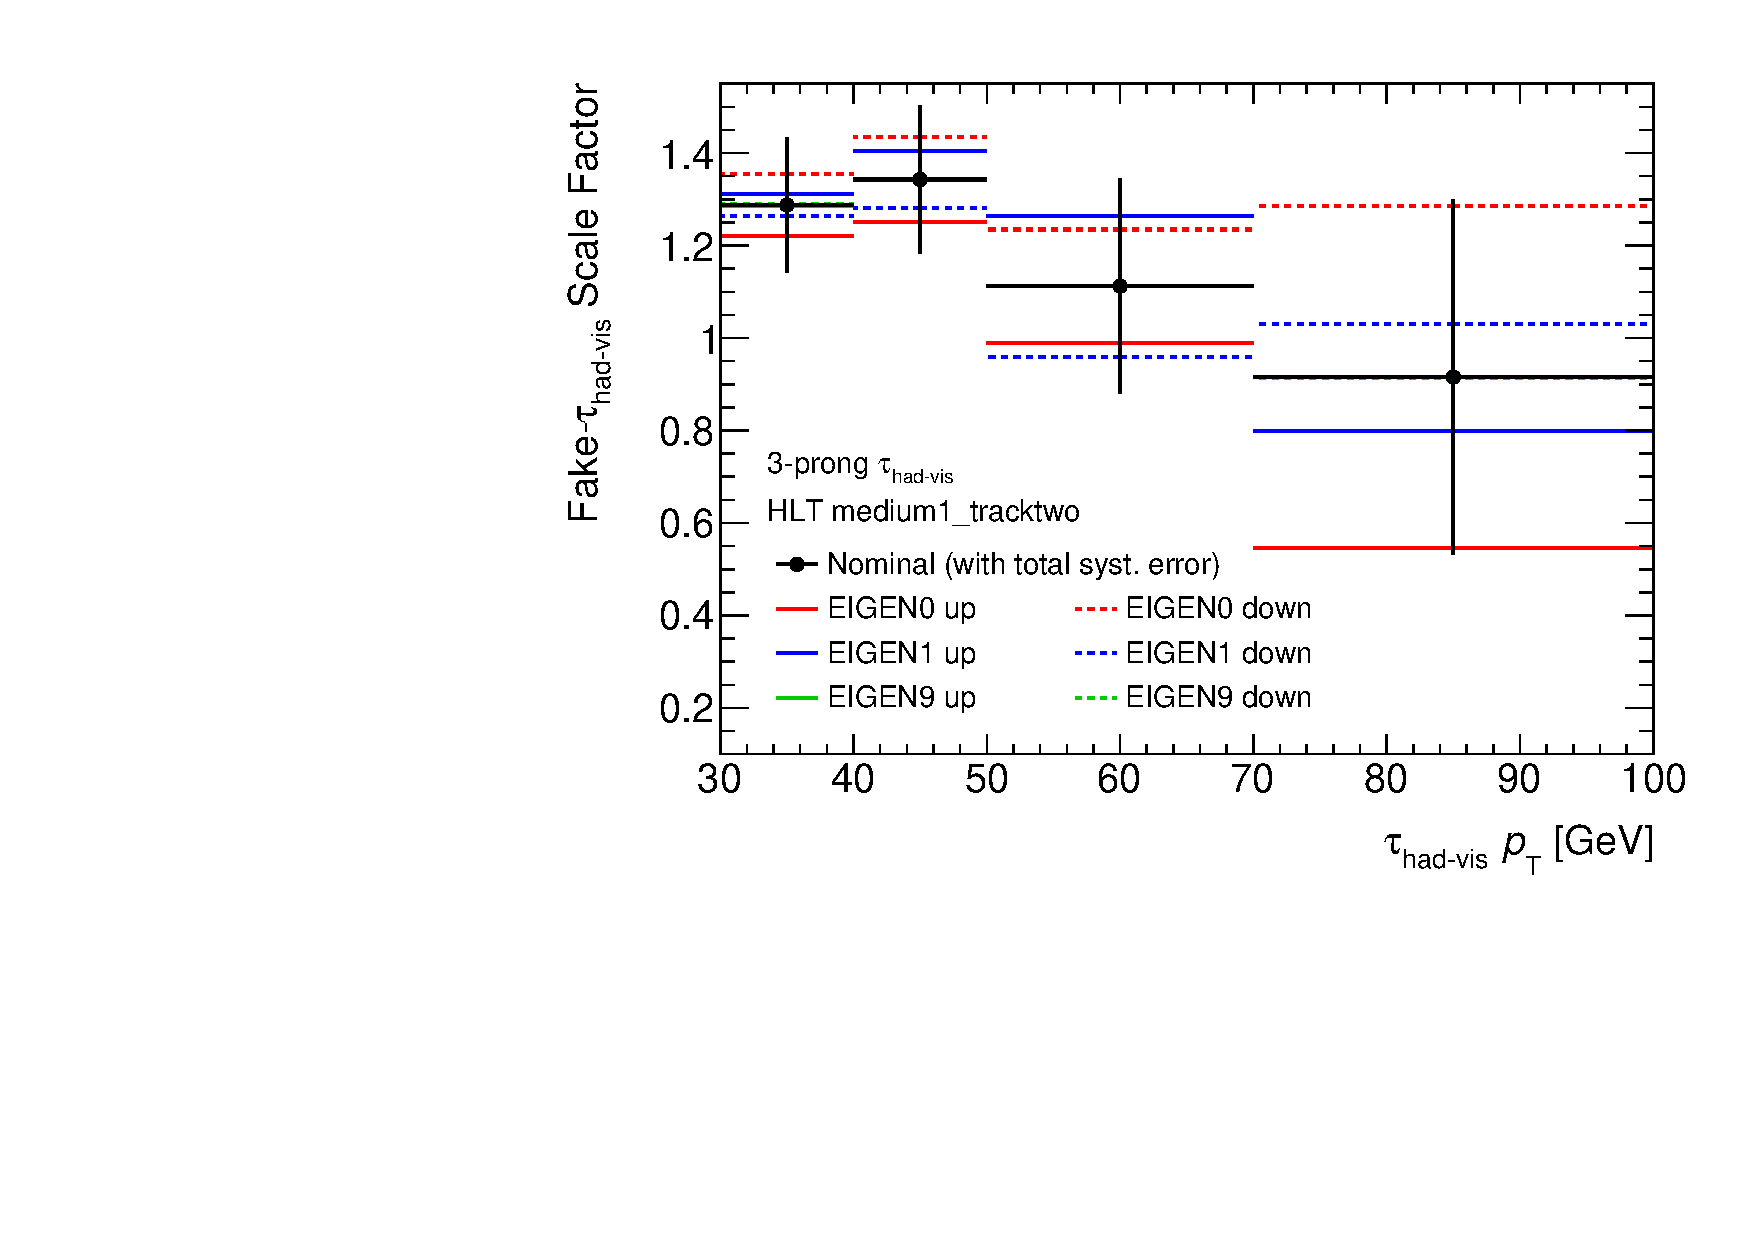
\includegraphics[width=\textwidth]{ttbarSF/ttbarSF_eigvar_3p}
    \caption{3-prong \tauhadvis}%
    \label{fig:ttbarSF_eigenvariations_3p}
  \end{subfigure}

  % Adding the deviations of all variations (\texttt{EIGEN0}--\texttt{EIGEN9})
  % from the nominal result in quadrature recovers the total uncertainty.

  \caption[Systematic variations of the \faketauhadvis SFs for the
  \texttt{HLT\_tau25\_medium1\_tracktwo} trigger.]{\Faketauhadvis SF variations
    resulting from the decorrelation procedure applied to the measurement for
    the \texttt{HLT\_tau25\_medium1\_tracktwo} trigger. The two variations
    leading in the explained variance (\texttt{EIGEN0} and \texttt{EIGEN1}) as
    well as the variation explaining the least variance (\texttt{EIGEN9}) are
    shown.}%
  \label{fig:ttbarSF_eigenvariations}
\end{figure}


\subsubsection{Application of \Faketauhadvis Scale Factors in the \hadhad
  Channel}

The \ttbarFakes background in the SR of the \hadhad channel is estimated by
applying \faketauhadvis SFs to \ttbar events from simulation with at least one
\faketauhadvis. These events are required to pass the SR selection criteria of
the \hadhad channel, including the trigger selection described
in~\Cref{sec:trigger}. The SFs are chosen depending on the trigger category and
whether the \faketauhadvis is the \tauhadvis candidate leading in \pT,
sub-leading in \pT, or both selected candidates are \faketauhadvis. When both
\tauhadvis candidates are originating from quark- or gluon-initiated jets, the
SF correction is assumed to factorise and the product of SFs is assigned as an
event-level weight.

In events selected by DTTs, both \tauhadvis candidates have to fulfil the
trigger-level identification requirements. In this case, the set of SFs is chosen
according to the trigger chain that selected the event, independent of which
\tauhadvis candidate is the \faketauhadvis. In contrast, only one \tauhadvis
candidate has to fulfil the trigger-level requirements in events selected by
STTs. For STT events, it is assumed that the \tauhadvis candidate leading in \pT
is the one satisfying the trigger conditions. This assumption is correct for
more than \SI{99}{\percent} of \ttbar events containing \faketauhadvis in the STT
category. Therefore, SFs measured for \faketauhadvis after trigger-matching are
applied when the leading \tauhadvis candidate is the \faketauhadvis; SFs derived
without trigger-matching are applied when the sub-leading \tauhadvis candidate
is the \faketauhadvis. Similar to the DTT case, if the \tauhadvis candidate
leading in \pT is the \faketauhadvis, then the set of SFs that corresponds to
the trigger chain that selected the event is used. The event weight calculation
is summarised in~\Cref{tab:ttbarSF_application_rule}.

\begin{table}[htbp]
  \centering

  \caption[Event weights for the application of SFs to \ttbarFakes events in
  simulation.]{Event weights for the application of SFs to \ttbarFakes events in
    simulation. Events are categorised by whether the leading \tauhadvis
    candidate~($\tau_{\text{lead.}}$), sub-leading \tauhadvis
    candidate~($\tau_{\text{subl.}}$), or both \tauhadvis candidates are
    \faketauhadvis. SFs for \faketauhadvis without identification at
    trigger-level are denoted by $\text{SF}_{\text{loose}}$. SFs for
    \faketauhadvis with both offline and trigger-level identification
    requirements are denoted by $\text{SF}_\text{loose+trig.}$.}%
  \label{tab:ttbarSF_application_rule}

  \resizebox{\textwidth}{!}{
    \begin{tabular}{cc@{\hskip 2em}rcl@{\hskip 2em}rcl}
  \toprule
  $\tau_{\text{lead.}}$ & $\tau_{\text{subl.}}$ & \multicolumn{3}{c}{Event weight (STT)} & \multicolumn{3}{c}{Event weight (DTT)} \\
  \midrule
  true & fake & $1$ & $\times$ & $\text{SF}_\text{loose}(\tau_{\text{subl.}})$
              & $1$ & $\times$ & $\text{SF}_\text{loose+trig.}(\tau_{\text{subl.}})$ \\[0.2em]

  fake & true & $\text{SF}_\text{loose+trig.}(\tau_{\text{lead.}})$ & $\times$ & $1$
              & $\text{SF}_\text{loose+trig.}(\tau_{\text{lead.}})$ & $\times$ & $1$ \\[0.2em]

  fake & fake & $\text{SF}_\text{loose+trig.}(\tau_{\text{lead.}})$ & $\times$ & $\text{SF}_\text{loose}(\tau_{\text{subl.}})$
              & $\text{SF}_\text{loose+trig.}(\tau_{\text{lead.}})$ & $\times$ & $\text{SF}_\text{loose+trig.}(\tau_{\text{subl.}})$ \\
  \bottomrule
\end{tabular}

%%% Local Variables:
%%% mode: latex
%%% TeX-master: "../phd_thesis"
%%% End:

  }
\end{table}


\subsubsection{Uncertainties on the \ttbarFakes Background in the \hadhad
  Channel}

In addition to the uncertainties originating from the SF measurement, two other
sources of uncertainties are considered. First, an uncertainty accounting for a
possible bias in the estimated SFs due to trigger efficiency turn-on effects
arising from \tauhadvis \pT (\ET) thresholds at the HLT (L1 trigger) is
determined. Second, an uncertainty on the extrapolation of the measured SFs from
$\ell + \tauhadvis$ final states to final states with two \tauhadvis is derived.

A systematic uncertainty accounting for the effect of \tauhadvis \pT (\ET)
thresholds at the HLT~(L1 trigger) on the \faketauhadvis SFs is estimated. The
nominal SF measurement is performed using \tauhadvis-triggers with thresholds of
$\pT > \SI{25}{\GeV}$ at the HLT and $\ET > \SI{12}{\GeV}$ at the L1
trigger~(\texttt{tau25}). However, triggers with higher thresholds are also
employed in the \hadhad channel. For example, thresholds of
$\pT > \SI{35}{\GeV}$ at the HLT and $\ET > \SI{20}{\GeV}$ at the L1 trigger
(\texttt{tau35}) are applied to the leading \tauhadvis candidate selected by
DTTs. The application of SFs measured for \texttt{tau25} triggers to
\faketauhadvis that are required to pass a \texttt{tau35} trigger can introduce
a bias due to differences in selection efficiency between both triggers. This
effect is only relevant for \faketauhadvis with transverse momenta close to the
\pT~threshold of the \texttt{tau35} trigger, i.e.\
\SIrange[range-phrase=--]{40}{50}{\GeV} for 1-prong candidates and
\SIrange[range-phrase=--]{40}{60}{\GeV} for 3-prong candidates. For
\faketauhadvis with larger transverse momenta, the differences between triggers
become negligible.

% The difference in trigger efficiency between \texttt{tau25} and \texttt{tau35}
% is studied in simulated \ttbarFakes events in the SF-CR. Only events with
% \tauhadvis candidates with $\pT > \SI{40}{\GeV}$ are considered. After this
% selection, \SI{95}{\percent} (\SI{85}{\percent}) of \faketauhadvis
% reconstructed as 1-prong (3-prong) candidates selected by \texttt{tau25} also
% pass the \texttt{tau35} triggers. The difference in \faketauhadvis selected by
% the \texttt{tau25} and \texttt{tau35} triggers is a potential source of bias
% in the estimation of the \ttbarFakes background. For \faketauhadvis
% reconstructed as 1-prong (3-prong) candidates and with $\pT > \SI{50}{\GeV}$
% ($\pT > \SI{60}{\GeV}$), the differences in \faketauhadvis selected by
% \texttt{tau25} and \texttt{tau35} become negligible.

An uncertainty is assigned to SFs applied to \faketauhadvis that are required to
pass a \texttt{tau35} trigger if the transverse momentum of the \faketauhadvis
is close to the \pT~threshold of the trigger. In particular, the uncertainty is
only applied for 1-prong (3-prong) \faketauhadvis with transverse momenta below
\SI{50}{\GeV} (\SI{60}{\GeV}). The size of the uncertainty is estimated by
repeating the SF measurement for the \texttt{tau35} triggers and comparing with
the nominal set of SFs. This comparison is performed for all trigger chains
employed in the analysis, resulting in a relative uncertainty of approximately
\SI{6}{\percent} for all triggers considered in this search.

% \begin{table}[htbp]
%   \centering

%   \caption{Size of the uncertainty comparing scale factors measured
%     for triggers with $\pTHLT > \SI{25}{\GeV}$ and
%     $\pTHLT > \SI{35}{\GeV}$ thresholds. The uncertainty is given
%     relative to all events from \ttbar in the \hadhad channel signal
%     region where the leading \tauhadvis is a \faketauhadvis with \pT
%     close to the \SI{40}{\GeV} threshold.}%
%   \label{tab:ttbarSF_tau25_35_uncertainty}

%   \begin{tabular}{lcc}
  \toprule
  & {1-prong \tauhadvis} & {3-prong \tauhadvis} \\
  & {(40 - 50 GeV)} & {(40 - 60 GeV)} \\
  \midrule
  \texttt{medium1\_tracktwo} (ttbarFT) & $\pm 5.8 \%$ & $\pm 5.5 \%$ \\
  \texttt{medium1\_tracktwo} (ttbarFF) & $\pm 5.9 \%$ & $\pm 5.2 \%$ \\[0.5em]

  \texttt{medium1\_tracktwoEF} (ttbarFT) & $\pm 6.4 \%$ & $\pm 8.1 \%$ \\
  \texttt{medium1\_tracktwoEF} (ttbarFF) & $\pm 6.4 \%$ & $\pm 8.0 \%$ \\[0.5em]

  \texttt{mediumRNN\_tracktwoMVA} (or EF) (ttbarFT) & $\pm 3.8 \%$ & $\pm 2.7 \%$ \\
  \texttt{mediumRNN\_tracktwoMVA} (or EF) (ttbarFF)& $\pm 4.0 \%$ & $\pm 2.6 \%$ \\
  \bottomrule
\end{tabular}

%%% Local Variables:
%%% mode: latex
%%% TeX-master: "../phd_thesis"
%%% End:

% \end{table}

The measurement of the SFs is performed in the SF-CR and applied to events in
the SR of the \hadhad channel. An uncertainty is assigned to account for the
extrapolation of the SFs from the SF-CR to the \hadhad SR. The
uncertainties are derived by performing variations of the \ttbar modelling in
simulation and comparing the acceptance of \ttbarFakes events in the SF-CR and
the \hadhad SR. Variations of the matrix element generator, the parton shower
simulation, the renormalisation and factorisation scales, and the modelling of
initial and final state radiation are considered
(cf.~\Cref{app:top_uncertainties}).

The comparison of \ttbarFakes acceptances are performed separately for events in
the \hadhad SR in which the leading \tauhadvis candidate is the \faketauhadvis
(FT~events), the sub-leading \tauhadvis candidate is the \faketauhadvis
(TF~events), and cases in which both candidates are \faketauhadvis
(FF~events). This comparison yields extrapolation uncertainties of
\SI{14}{\percent} for TF~events, \SI{7}{\percent} for FT~events, and
\SI{39}{\percent} for the FF~events. In all cases, the uncertainty is dominated
by the comparison of \PYTHIA[8] and \HERWIG[7] for the simulation of the parton
shower. The large uncertainty on FF~events is expected since the measurement in
the SF-CR can only target events with exactly one \faketauhadvis.

% \begin{align*}
%   N(\ttbarFakes) = \num{2490}
%   \valuesep\numerrt{22}{stat.}%
%   \valuesep\numerrt{210}{meas.}%
%   \valuesep\numerrt{240}{extrapol.}%
%   \valuesep\numerrt{3.6}{trigger threshold} \,\text{.}
% \end{align*}
In the following, the impact of the uncertainties on the total \ttbarFakes
background prediction in the SR of the \hadhad channel is summarised. The
relative uncertainties on the prediction split by uncertainty source are:
\begin{itemize}

\item Uncertainties from the SF measurement:~$\pm \SI{8.5}{\percent}$.

\item Extrapolation uncertainties (SF-CR $\ra$ \hadhad
  SR):~$\pm \SI{9.7}{\percent}$.

\item Uncertainty on SFs due to different \pT (\ET) thresholds of
  \tauhadvis-triggers:~$\pm \SI{0.2}{\percent}$.

\item Statistical uncertainty from finite number of simulated
  events:~$\pm \SI{0.9}{\percent}$.

\end{itemize}
The dominant sources of uncertainty on the prediction of the \ttbarFakes
background are the uncertainties on the SFs from the SF measurement and the
extrapolation uncertainties. Due to the small expected number of FF events in
the \hadhad SR (cf.~\Cref{tab:ttbarSF_yields}), the large extrapolation
uncertainty for FF events has limited impact on the uncertainty of the total
\ttbarFakes prediction.
% The uncertainty accounting for the effects of different \pT~(\ET)~thresholds
% of \tauhadvis-triggers has only a minor impact on the overall \ttbarFakes
% background prediction since only a small fraction of events is affected by
% this uncertainty.
\Cref{tab:ttbarSF_yields} summarises the \ttbarFakes prediction in the \hadhad
SR and compares it to the prediction from simulation without application of
\faketauhadvis SFs.
% Generally, both predictions agree within uncertainties except for the
% FT~component. The predicted number of FT~events is smaller after application
% of \ttbarFake SFs due to SFs being smaller than unity for \faketauhadvis with
% high~\pT.

% The total \ttbarFakes event yield in the \hadhad SR is determined with a
% relative uncertainty of \SI{13}{\percent}, agreeing with the uncorrected
% estimate of the total yield within uncertainties. The expected number of
% \ttbarFakes events is slightly smaller after correction since the measured
% scale factors for high \pT \faketauhadvis tend to be smaller than unity. This
% is also reflected in the larger relative change of the the FT-component (the
% leading \tauhadvis candidate is a \faketauhadvis), for which the
% \faketauhadvis has an average \pT of \SI{65}{\GeV}.

% The SF method described in this section provides a measurement-driven approach
% of estimating the \ttbarFakes background and its uncertainty in the SR of the
% \hadhad channel.  In~\Cref{tab:ttbarSF_yields}, the event yield of \ttbarFakes
% in the \hadhad SR is shown and compared to \ttbar simulation without
% corrections.

\begin{table}[htbp]
  \centering

  % The \ttbarFakes background is split into cases where the sub-leading
  % \tauhadvis candidate is the \faketauhadvis (TF), the leading \tauhadvis
  % candidate is the \faketauhadvis, or both candidate are \faketauhadvis (FF).

  \caption[Expected number of \ttbarFakes events in the \hadhad SR with and
  without application of the \faketauhadvis~SFs.]{Expected number of \ttbarFakes
    events in the \hadhad SR with (right) and without (left) application of the
    \faketauhadvis~SFs. Only MC statistical uncertainties are shown for the
    estimate without application of the \faketauhadvis~SFs. The background
    estimate using the \faketauhadvis~SFs includes statistical uncertainties and
    all systematic uncertainties related to the SF method. Other experimental
    uncertainties are omitted.}%
  \label{tab:ttbarSF_yields}

  % Source:
% https://docs.google.com/spreadsheets/d/1uwVElPaR1HuqEHaL8eAh5pEoGdK2ZBQ8D_Ob8lSSPwE/edit#gid=0

% fSumw[1]=2705.09, x=0.5, error=22.9788

% Only measurement uncertainties
% ttbarSFTF: 1433.95 +- 87.88
% ttbarSFFT: 698.52 +- 72.21
% ttbarSFFF: 358.92 +- 53.50
% Total: 2491.39 +- 21.59 +- 202.99 = 204.13493

\begin{tabular}{
  l
  @{\hskip 16pt}
  S[table-format=4.0(2)]
  @{\hskip 16pt}
  S[table-format=4.0(3)]
  }
  \toprule
  & \multicolumn{2}{c}{Expected number of events (pre-fit)} \\
  \cmidrule{2-3}
          & {Simulation} & {Simulation with} \\
  Process &              & {\faketauhadvisC SF}  \\
  \midrule
  \ttbar + \faketauhadvisC (TF) & 1428 +- 16 & 1430 +- 230 \\
  \ttbar + \faketauhadvisC (FT) & 854 +- 13 & 699 +- 88 \\
  \ttbar + \faketauhadvisC (FF) & 423 +- 12 & 360 +- 160 \\
  \midrule
  \ttbar + \faketauhadvisC (total) & 2705 +- 23 & 2490 +- 320 \\
  \bottomrule
\end{tabular}

%%% Local Variables:
%%% mode: latex
%%% TeX-master: "../phd_thesis"
%%% End:

\end{table}

% The uncertainties originating from the SF measurement in the SF-CR (meas.) and
% the extrapolation uncertainties (extrapol.) have uncertainties of similar
% size. The extrapolation uncertainty is dominated by the comparison of
% different parton shower programs. The \faketauhadvis \pT-dependent PS
% uncertainty, affecting the TF- and FT-components of the background, has a
% particularly large impact on the TF contribution. This is due to the large
% uncertainty for 1-prong \faketauhadvis candidates, making up $\frac{3}{4}$ of
% \faketauhadvis in \ttbar, at low transverse momenta as shown
% in~\Cref{fig:ttbarSF_extrapol_shape_a}. Due to the momentum ordering, the
% average \faketauhadvis \pT in \ttbarFakes (TF) is approximately \SI{40}{\GeV}.

% Statistical uncertainties from the finite number of simulated events (stat.)
% and the uncertainty based on the comparison of different trigger thresholds
% (trigger threshold) have negligible impact on the total yield in the \hadhad
% SR.

% Measurement uncertainties on total yield are highly correlated: ca.
% 90% PS uncertainty for 1-prong taus is anti-correlated due to sign-change of uncertainty


\subsubsection{Estimation of \Faketauhadvis Scale Factors for Anti-\tauhadvis}

The estimation of the \multijet background in the \hadhad SR, which is described
in~\Cref{sec:bkg_hadhad_ff}, requires a large subtraction of \ttbarFakes events
in a region defined by the presence of an \antitau
(cf.~\Cref{sec:object_reconstruction}). The SF method is extended to \antitau to
provide uncertainties on this subtraction.
% in the 2 $b$-tag \antiid CR for \tauhadvis candidates with OS electric
% charge. The SF method for estimating the \ttbarFakes background is extended to
% the \antiid region to provide uncertainties on the subtraction performed as
% part of the \multijet estimation.

The SF measurement is repeated using the same SF-CR definition except for
requiring an \antitau instead of a \tauhadvis candidate passing loose
identification.
% inverting the \tauhadvis identification requirement applied during offline
% event reconstruction. Instead of \tauhadvis passing the loose \tauid working
% point, \tauhadvis are required to fail the loose working point but exceed an
% RNN \tauid score threshold of \num{0.01}. The same requirements from the
% ID-region measurement regarding the reconstruction and identification of
% \tauhadvis at the HLT are imposed.\todo{Already explained (object selection)}
This inversion of the \tauid requirement rejects most \ttbar events with
true-\tauhadvis, yielding a region with \ttbarFakes purity of about
\SI{80}{\percent}. Trigger-matching of the \antitau to a \tauhadvis at the HLT
reduces the \ttbarFakes yield by about \SI{80}{\percent} due to the
trigger-level identification requirements; however, only a mild decrease in
\ttbarFakes purity by about 5 percentage points is observed.
% remains largely unchanged.

A reduced set of experimental uncertainties is used for this measurement due to
practical limitations in the dataset preparation for the
$\ell + \text{anti-}\tauhadvis$ region. Uncertainties varying the four-momentum
of reconstructed objects are omitted except uncertainties on the \tauhadvis
energy scale. Other uncertainties that can be expressed as alternative event
weights, for example uncertainties on tagging efficiencies, are considered. Due
to this constraint, the total deviation of the central value of the SFs from
unity is assigned as an additional uncertainty on the measured SFs for \antitau.

The measured SFs for \antitau are shown in~\Cref{fig:ttbarSF_antiid_SF}. The SFs
are generally within \SI{20}{\percent} of unity. The same decorrelation
technique is used to propagate the measurement uncertainties when applying the
SFs to \antitau in the \hadhad channel. The context and impact of the SFs for
\antitau on the \multijet estimate is discussed in \Cref{sec:bkg_hadhad_ff}.

\begin{figure}[htbp]
  \centering

  \begin{subfigure}[t]{.495\textwidth}
    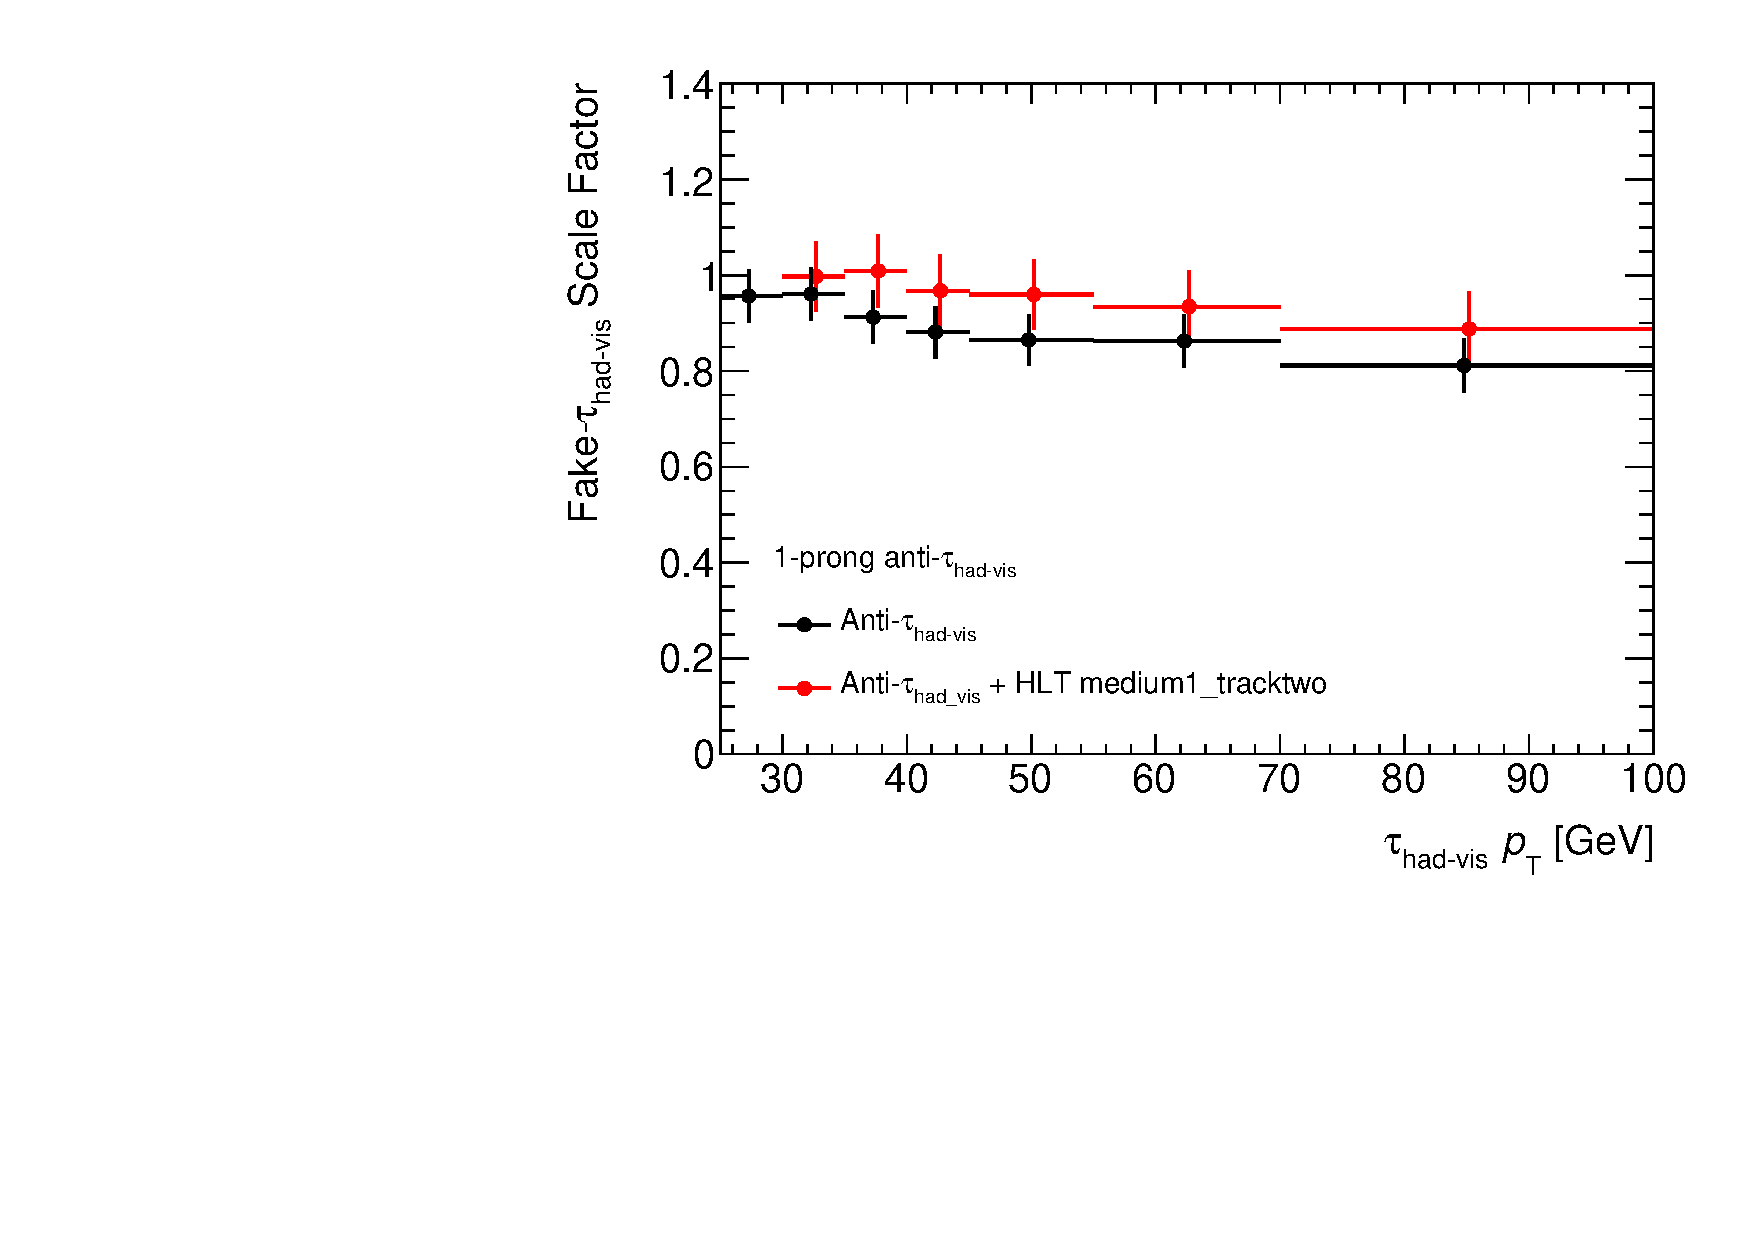
\includegraphics[width=\textwidth]{ttbarSF/scale_factors/ttbarSF_antitau_offl_tau25_1p}
    \caption{}
    \label{fig:ttbarSF_antiid_SF_a}
  \end{subfigure}\hfill%
  \begin{subfigure}[t]{.495\textwidth}
    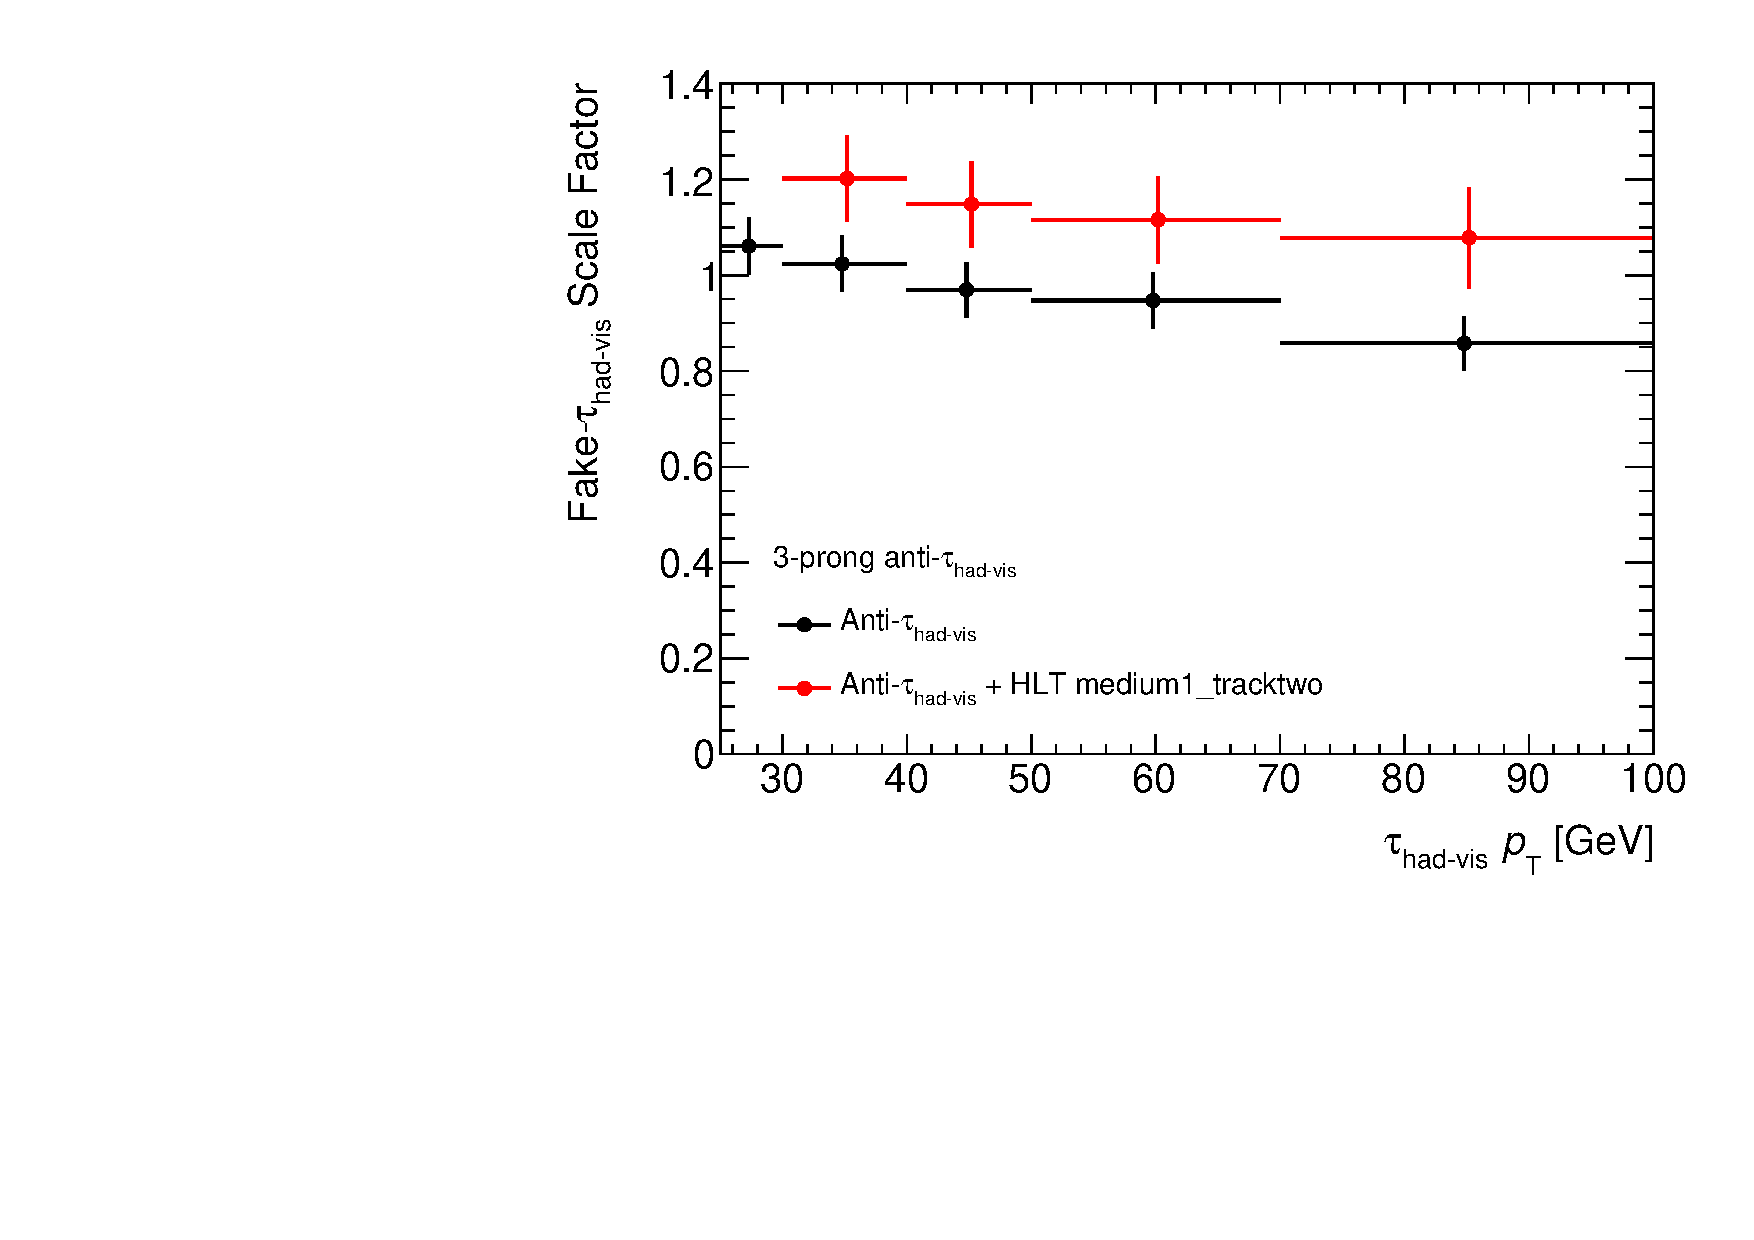
\includegraphics[width=\textwidth]{ttbarSF/scale_factors/ttbarSF_antitau_offl_tau25_3p}
    \caption{}
    \label{fig:ttbarSF_antiid_SF_b}
  \end{subfigure}

  \begin{subfigure}[t]{.495\textwidth}
    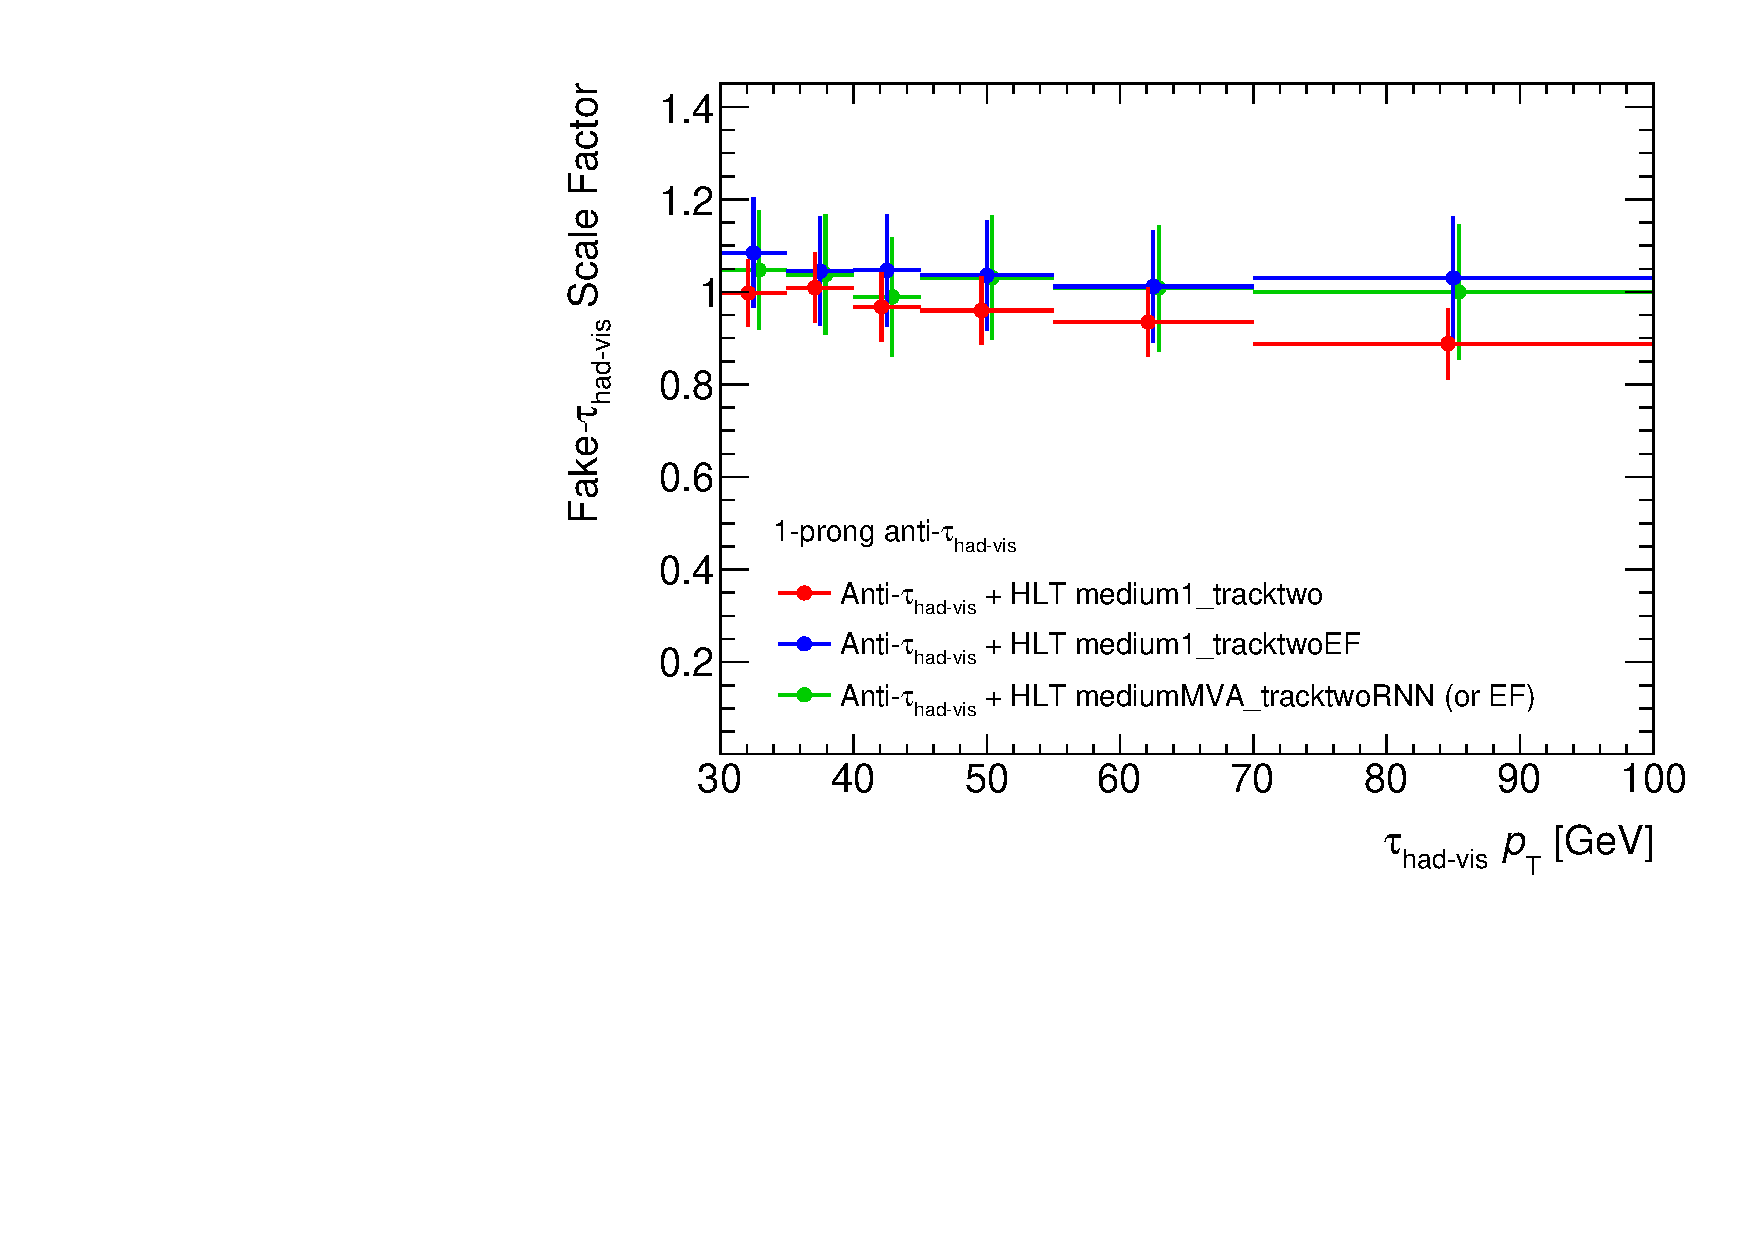
\includegraphics[width=\textwidth]{ttbarSF/scale_factors/ttbarSF_antitau_tau25_1p}
    \caption{}
    \label{fig:ttbarSF_antiid_SF_c}
  \end{subfigure}\hfill%
  \begin{subfigure}[t]{.495\textwidth}
    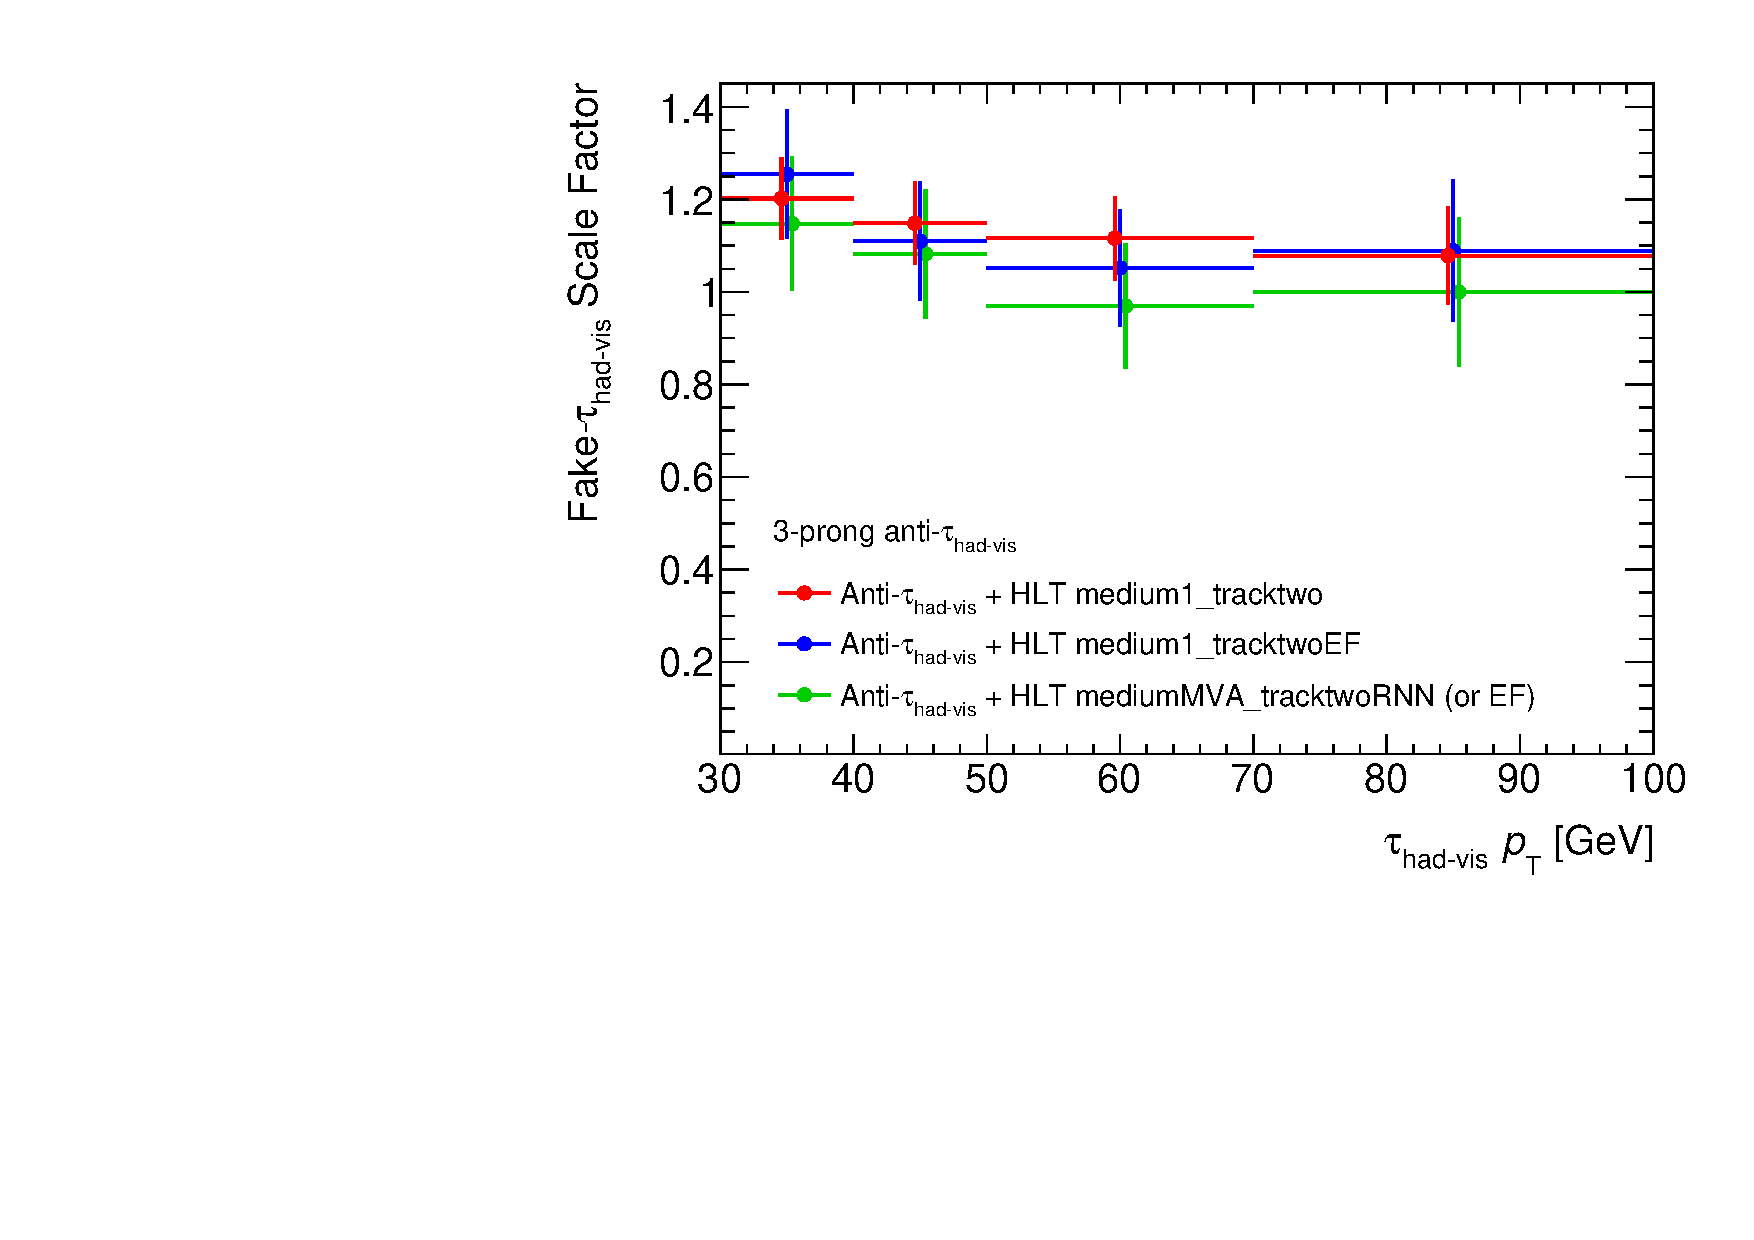
\includegraphics[width=\textwidth]{ttbarSF/scale_factors/ttbarSF_antitau_tau25_3p}
    \caption{}
    \label{fig:ttbarSF_antiid_SF_d}
  \end{subfigure}

  \caption[\Faketauhadvis SFs for anti-\tauhadvis and different \tauid criteria
  applied at trigger-level.]{\Faketauhadvis SFs for anti-\tauhadvis and
    different \tauid criteria applied at trigger-level. Figures~(a) and~(b)
    compare the SFs with and without \tauid at the HLT. The effect of different
    \tauhadvis-triggers on the extracted SFs is shown in~(c) and~(d). The last
    bin summarises events with \tauhadvis~$\pT \geq \SI{70}{\GeV}$. The markers
    are shifted from the geometrical bin centre for illustration purposes
    only. The depicted SFs include all statistical and systematic
    uncertainties.}%
  \label{fig:ttbarSF_antiid_SF}
\end{figure}

%%% Local Variables:
%%% mode: latex
%%% TeX-master: "../../phd_thesis"
%%% End:
